\hypertarget{sec:solution}{%
\chapter{Addressing Effort and Risk Concerns in Web Migration}\label{sec:solution}}
This chapter outlines the \gls{awsm} (Agile Web Migration for \glspl{sme}) \autocite{Heil2016AWSM} approach providing a solution to address the shortcomings summarized in \cref{g:1}, \cref{g:2}, and \cref{g:3} which were identified in the state of the art of \gls{Web Migration} that keep \glspl{isv}, in particular \gls{sme}-sized \glspl{isv}, from commencing a \gls{Web Migration}.
To devise a suitable solution addressing these gaps, \cref{sec:research-objectives} identifies the main research objectives of this thesis.
\Cref{sec:solution-overview} derives the  \gls{awsm} solution achieving these research objectives, consisting of the \gls{awsm} Methodology and Toolsuite.

\vspace{-15pt}
\hypertarget{sec:research-objectives}{%
\section{Research Objectives}\label{sec:research-objectives}}
\vspace{15pt}

As identified in \cref{sec:sota.shortcomings}, \gls{Web Migration} research currently lacks in three areas: the feasibility with limited resources and limited migration and \gls{target environment} expertise (\cref{g:1}), the demonstration of desirability for decision making and risk management in initial phases (\cref{g:2}), and the user interface migration and user interaction reuse (\cref{g:3}).
These gaps correspond to the \emph{doubts about feasibility} and \emph{doubts about desirability} for \glspl{isv} with non-\glslink{web}{Web}\glspl{Legacy System} and large existing user bases observed in the scenario in \cref{sec:problem-analysis-results}.
In order to devise a solution that addresses the gaps and supports \glspl{isv} to commence \gls{Web Migration}, a set of research objectives that outline suitable key solution characteristics for the stakeholder-specific problems needs to be derived.
To drive ideation of solution ideas that represent research objectives, the \emph{How-Might-We} method of \gls{hcd} is applied.
\gls{hmw} questions were formulated in a collaborative \emph{brainstorm} session.
The initial \gls{hmw} question was:

\begin{quote}
How might we address IVS's doubts about feasibility and desirability?
\end{quote}

By considering the three main gaps in the state of the art of \gls{Web Migration} in \cref{sec:sota.shortcomings} and the detailed problem in \cref{sec:problem-analysis-results}, this question is further broken down into the HMW questions listed in \cref{tbl:hmw}. 

\hypertarget{tbl:hmw}{}
\begin{longtable}[]{@{}ll@{}}
\caption[How-Might-We-Questions for Research Objective Ideation]{\label{tbl:hmw}How-Might-We-Questions for Ideation of Research Objectives}\tabularnewline
\toprule
\begin{minipage}[b]{0.1\columnwidth}\raggedright
ID\strut
\end{minipage} & \begin{minipage}[b]{0.84\columnwidth}\raggedright
HMW-Question: \emph{How might we...}\strut
\end{minipage}\tabularnewline
\midrule
\endfirsthead
\toprule
\begin{minipage}[b]{0.1\columnwidth}\raggedright
ID\strut
\end{minipage} & \begin{minipage}[b]{0.84\columnwidth}\raggedright
Question\strut
\end{minipage}\tabularnewline
\midrule
\endhead
\begin{minipage}[t]{0.1\columnwidth}\raggedright
HMW1\strut
\end{minipage} & \begin{minipage}[t]{0.84\columnwidth}\raggedright
reduce the risk of loss of knowledge through \gls{Web Migration}?\strut
\end{minipage}\tabularnewline
\begin{minipage}[t]{0.1\columnwidth}\raggedright
HMW2\strut
\end{minipage} & \begin{minipage}[t]{0.84\columnwidth}\raggedright
demonstrate feasibility and advantages of a \web-based version of the \gls{Legacy System}?\strut
\end{minipage}\tabularnewline
\begin{minipage}[t]{0.1\columnwidth}\raggedright
HMW3\strut
\end{minipage} & \begin{minipage}[t]{0.84\columnwidth}\raggedright
reduce the risk of customers impact through \gls{Web Migration}?\strut
\end{minipage}\tabularnewline
\begin{minipage}[t]{0.1\columnwidth}\raggedright
HMW4\strut
\end{minipage} & \begin{minipage}[t]{0.84\columnwidth}\raggedright
address HMW1, HMW2 and HMW3 with limited resources and lack of \gls{Web Engineering} expertise?\strut
\end{minipage}\tabularnewline
\bottomrule
\end{longtable}

\vspace{-15pt}
Questions HMW1 - HMW3 address the problems of feasibility and desirability doubts relating to \cref{g:2} and \cref{g:3} from a \emph{functional} \autocite{ISO/IEEE24765Vocabulary} perspective.
HMW4 is a \emph{non-functional} \autocite{ISO/IEEE24765Vocabulary} cross-cutting constraint, representing the resource and expertise problems in \cref{g:1} and therefore is integrated with all following research objectives.
The overarching goal of this thesis is:

\vspace{-15pt}
\begin{overarchinggoal}{og}
To provide methods, models, and tools that support \glspl{isv} with limited resources and lack of \gls{Web Engineering} expertise to commence a \gls{Web Migration}.
\end{overarchinggoal}

To achieve this goal, three specific research objectives are identified from the \gls{hmw} questions in \cref{tbl:hmw} employing \gls{hcd}-based opportunity ideation.
These objectives are:

\begin{researchobjective}{ro:1}
To enable identification and management of existing knowledge in legacy source code with limited resources and lack of \gls{Web Engineering} expertise.
\end{researchobjective}

\begin{researchobjective}{ro:2}
To enable demonstration of desirability and feasibility of a potential \glslink{web}{Web}-based version of the \gls{Legacy System} with limited resources and lack of \gls{Web Engineering} expertise.
\end{researchobjective}

\begin{researchobjective}{ro:3}
To enable control of the impact of user interface changes through \gls{Web Migration} on customers with limited resources and lack of \gls{Web Engineering} expertise.
\end{researchobjective}

Each research objective addresses at least one of the gaps identified in \cref{sec:sota.shortcomings} as visualized in \cref{fig:gaps-ro}
The solution specified in the following section addresses these three research objectives.

\begin{figure}[hbt]
\hypertarget{fig:gaps-ro}{%
\centering%
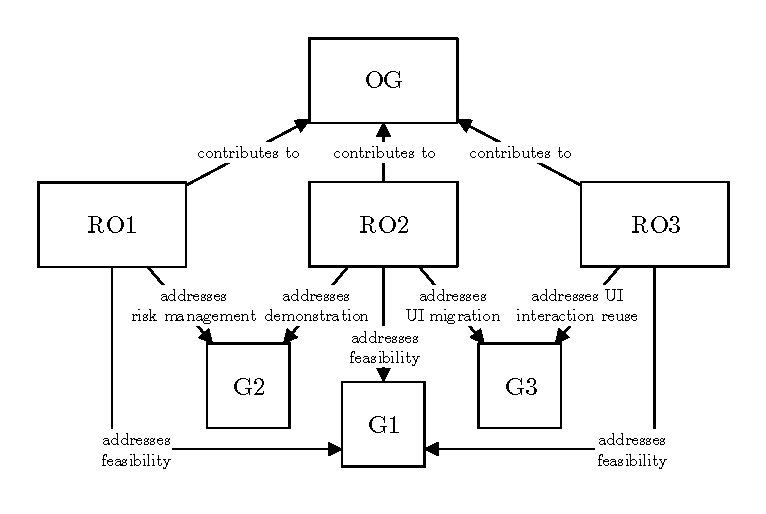
\includegraphics[width=0.75\textwidth]{../figures/gaps-ro.pdf}%
\caption{Relationships between Research Objectives and Gaps}%
\label{fig:gaps-ro}%
}
\end{figure}

The solution ideas corresponding to the research objectives were communicated by \emph{visual} representations (cf.~paper prototypes in \cref{sec:re.impl.integration}) and software \emph{prototypes}.
\gls{hcd} \emph{Feedback Integration and Iteration} was used to improve the solution ideas through stakeholder feedback gathered in a presentation and discussion session at the \glspl{isv} headquarters and continued throughout the entire research project.
%Eventually, the specific research questions presented at the beginning of \cref{sec:awsm-re,sec:awsm-rm,sec:awsm-ci} were derived which define the solution parts on a coarse-grain level.
%The resulting solution \& research design is described in \cref{sec:solution-overview}.


%\begin{figure}
%\hypertarget{fig:objectives}{%
%\centering
%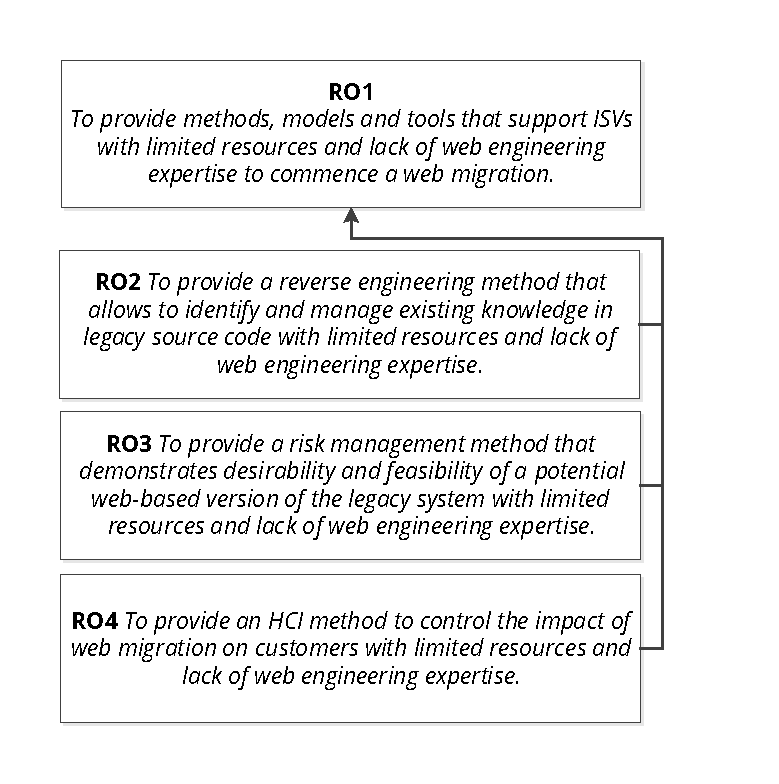
\includegraphics[width=0.99\textwidth]{../figures/objectives.pdf}
%\caption{Research Objectives}\label{fig:objectives}
%}
%\end{figure}

\vspace{-20pt}
\hypertarget{sec:solution-overview}{%
\section{Overview}\label{sec:solution-overview}}
\vspace{10pt}

Our solution to address \cref{ro:1} to \cref{ro:3} is \emph{\gls{awsm} (Agile Web Migration for \glspl{sme})} \autocite{Heil2016AWSM}.
\gls{awsm} addresses shortcomings of existing \gls{Web Migration} approaches in initial phases of migration projects.

To achieve this, it provides solutions for each of the research objectives representing the three \textbf{\gls{awsm} Methods}:

\begin{itemize}
\item the \gls{awsm} Reverse Engineering Method for \cref{ro:1},
\item the \gls{awsm} Risk Management Method for \cref{ro:2}, and
\item the \gls{awsm} Customer Impact Control Method for \cref{ro:3}.
\end{itemize}


\gls{awsm} is structured according to the constructive elements of software engineering for quality ensurance \autocite{Wallmueller2001SoftwareQuality} into Methods, Tools, Principles, and Formalisms.
\Cref{fig:solution} shows the overall architecture of \gls{awsm}.
The Methods, Tools, Principles, and Formalisms are grouped into two main parts: the \gls{awsm} Methodology, and the \gls{awsm} Toolsuite.
%\begin{itemize}
%\item \gls{awsm} Methodology, and the
%\item \gls{awsm} Toolsuite.
%\end{itemize}

\begin{figure}[h!]
\hypertarget{fig:solution}{%
\centering
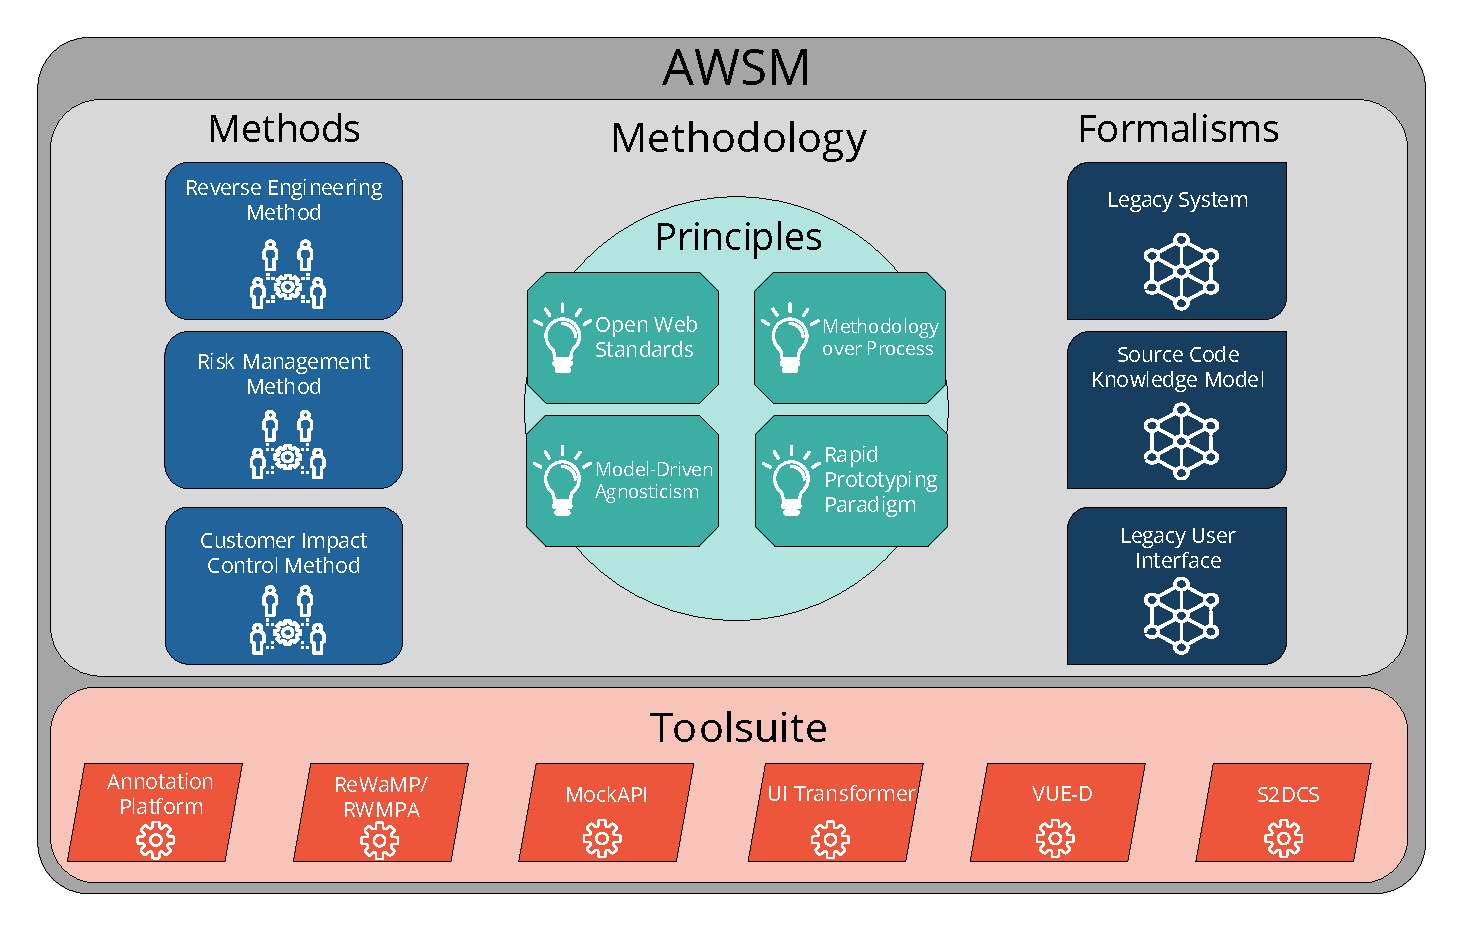
\includegraphics[width=0.99\textwidth]{../figures/solution2-defense.pdf}
\caption{AWSM Solution Overview}\label{fig:solution}
}
\end{figure}

The \gls{awsm} Methodology describes \gls{awsm}'s Methods, Principles, and Formalisms.
The Tools supporting the \gls{awsm} Methodology constitute the \gls{awsm} Toolsuite.
%Like other migration support methodologies  \autocite{Lewis2008SMART,Lewis2005SMART}, 
\gls{awsm} does not impose a specific migration process.
Thus, the \gls{awsm} Methodology focuses on principles, formalisms, and methods for \gls{Web Migration} initiation and integration with existing comprehensive migration methods.
\gls{awsm} can be combined with incremental \gls{Reengineering} and \gls{Transformation} processes, addressing the widely used package-oriented, feature-driven incremental migration process model characterized in \cref{sec:sota.discussion.crosscutting}.
For selecting or creating a suitable migration approach, \gls{awsm} provides a decision support system, as described in \cref{sec:s2dcs}.

The \gls{awsm} Methods are integrated into the selected migration approach, as shown in \cref{fig:methods-techniques-tools}.
For consistent description, we apply the taxonomy from the \gls{remip} reference model \autocite{Sneed2010SoftwareMigration} throughout this thesis.
The migration approach is divided into distinct sequential or parallel \emph{migration phases}.
These phases comprise at least one \emph{migration activity} which employs one or more \emph{migration methods}.
The three methods of the \gls{awsm} Methodology described in the following provide solutions to address the identified gaps in current \gls{Web Migration} approaches through integration at the activity level.
For each \gls{awsm} Method, at least one \emph{migration technique} is specified, detailing how to conduct a part of the method.

\textbf{\gls{awsm} Tools} support each technique and are the parts of the \gls{awsm} Toolsuite.
\textbf{\gls{awsm} Principles} are at the foundation of \gls{awsm}.
They are derived from the requirements and state of the art analysis results, and represent top-level design decisions of the \gls{awsm} Methodology and Toolsuite.
\textbf{\gls{awsm} Formalisms} form the conceptual basis for the Methods and Tools.
They specify the underlying model and semantics for knowledge in \glslink{Legacy System}{legacy} source code and the definition and algorithm for measuring the similarity between original and migrated user interfaces.
The following four subsections describe the solutions provided by the \gls{awsm} Methods, Tools, Principles, and Formalisms.

\begin{figure}[h!]
\hypertarget{fig:methods-techniques-tools}{%
\centering
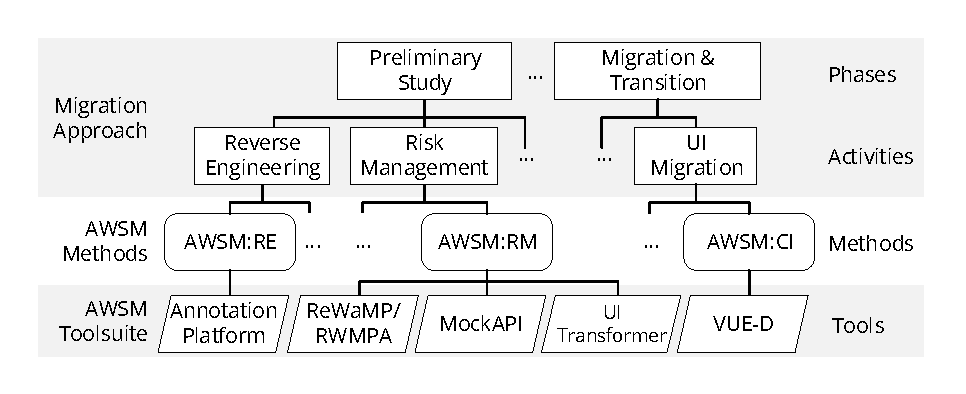
\includegraphics[width=0.98\textwidth]{../figures/methods-context.pdf}
\caption[AWSM in Context]{AWSM in Context, mapped to \gls{remip} Taxonomy}\label{fig:methods-techniques-tools}
}
\end{figure}

\vspace{-12pt}
\hypertarget{sec:solution.methods}{%
\section{Methods}\label{sec:solution.methods}}
\vspace{11pt}

To address the research objectives, \gls{awsm} provides three methods:
\begin{itemize}
\item AWSM:RE -- the \gls{awsm} Reverse Engineering Method,
\item AWSM:RM -- the \gls{awsm} Risk Management Method,
\item AWSM:CI -- the \gls{awsm} Customer Impact Control Method.
\end{itemize}

These three methods provide techniques for solving the problems identified in \cref{sec:sota.shortcomings} in different  disciplines and phases of \gls{Web Migration}.
While the techniques of AWSM:RE and AWSM:RM belong to the initial phase, AWSM:CI techniques are conducted during Migration \& Transition.
The three methods cover several core and base disciplines each, but all are targeting the migration decision milestone.
\Cref{tbl:awsm-remip} provides an overview mapping of the \gls{awsm} Methods mapping them onto the migration phases and disciplines of the Reference Migration Process \autocite{Sneed2010ReMiP} in order to facilitate integration with existing \gls{Web Migration} approaches. % as per principle \cref{p:2}.
The following three subsections outline the three AWSM Methods.

\hypertarget{tbl:awsm-remip}{}
\begin{longtable}[]{@{}l@{\phantom{AAAAA}}l@{}l@{}l@{}}
\caption{\label{tbl:awsm-remip}Mapping of AWSM Methods to \gls{remip}}\tabularnewline
\toprule
\begin{minipage}[b]{0.07\columnwidth}\raggedright
Method\strut
\end{minipage} & \begin{minipage}[b]{0.2\columnwidth}\raggedright
Phase\strut
\end{minipage} & \begin{minipage}[b]{0.25\columnwidth}\raggedright
Core Disciplines\strut
\end{minipage} & \begin{minipage}[b]{0.37\columnwidth}\raggedright
Base Disciplines\strut
\end{minipage}\tabularnewline
\midrule
\endfirsthead
\toprule
\begin{minipage}[b]{0.07\columnwidth}\raggedright
Method\strut
\end{minipage} & \begin{minipage}[b]{0.2\columnwidth}\raggedright
Phase\strut
\end{minipage} & \begin{minipage}[b]{0.25\columnwidth}\raggedright
Core Disciplines\strut
\end{minipage} & \begin{minipage}[b]{0.37\columnwidth}\raggedright
Base Disciplines\strut
\end{minipage}\tabularnewline
\midrule
\endhead
\begin{minipage}[t]{0.07\columnwidth}\raggedright
AWSM:RE\strut
\end{minipage} & \begin{minipage}[t]{0.2\columnwidth}\raggedright
Preliminary Study\strut
\end{minipage} & \begin{minipage}[t]{0.25\columnwidth}\raggedright
Legacy Analysis, Requirements Analysis\strut
\end{minipage} & \begin{minipage}[t]{0.37\columnwidth}\raggedright
Configuration \& Change Management, Project Management, Migration Environment\strut
\end{minipage}\tabularnewline
\begin{minipage}[t]{0.07\columnwidth}\raggedright
AWSM:RM\strut
\end{minipage} & \begin{minipage}[t]{0.2\columnwidth}\raggedright
Preliminary Study\strut
\end{minipage} & \begin{minipage}[t]{0.25\columnwidth}\raggedright
Requirements Analysis, Target Design\strut
\end{minipage} & \begin{minipage}[t]{0.37\columnwidth}\raggedright
Project Management, Staff Qualification\strut
\end{minipage}\tabularnewline
\begin{minipage}[t]{0.07\columnwidth}\raggedright
AWSM:CI\strut
\end{minipage} & \begin{minipage}[t]{0.2\columnwidth}\raggedright
Migration \& Transition\strut
\end{minipage} & \begin{minipage}[t]{0.25\columnwidth}\raggedright
Target Design, Implementation\strut
\end{minipage} & \begin{minipage}[t]{0.37\columnwidth}\raggedright
Migration Environment\strut
\end{minipage}\tabularnewline
\bottomrule
\end{longtable}

\vspace{-10pt}
\hypertarget{awsm-reverse-engineering-method}{%
\subsection{AWSM Reverse Engineering Method}\label{awsm-reverse-engineering-method}}
\vspace{10pt}

\begin{figure}[h!]
\hypertarget{fig:solution-re}{%
\centering
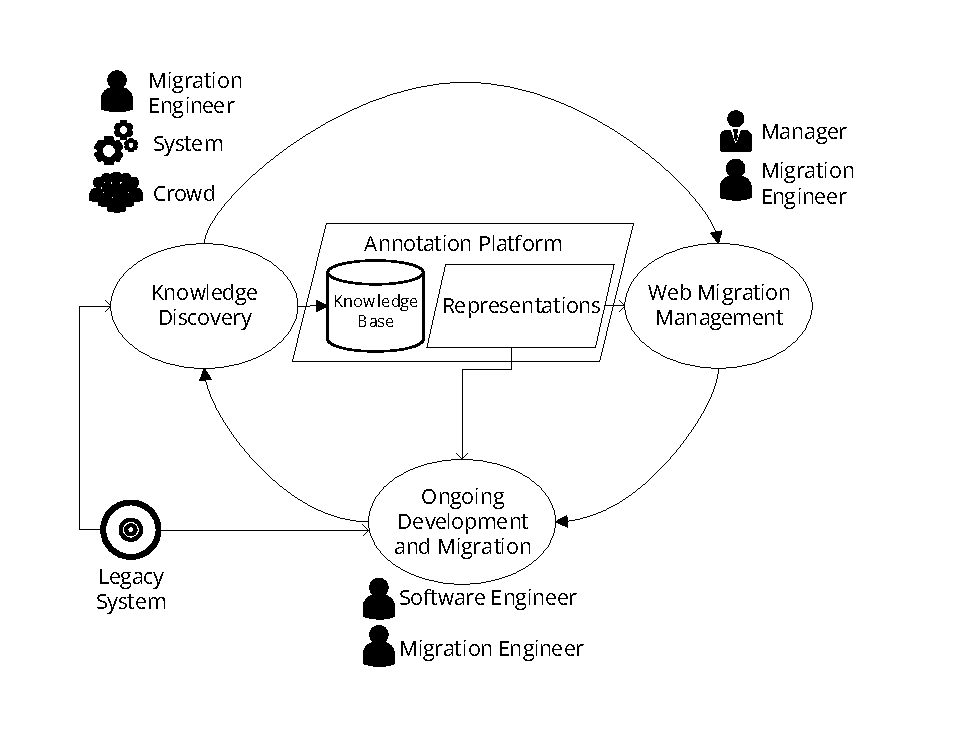
\includegraphics[width=0.98\textwidth]{../figures/solution-re.pdf}
\caption{AWSM:RE Method Overview}\label{fig:solution-re}
}
\end{figure}

The AWSM Reverse Engineering Method (AWSM:RE) shown in \cref{fig:solution-re} provides a solution for \cref{ro:1} by specifying techniques to identify and manage problem and solution domain knowledge in \glslink{Legacy System}{legacy} source code.
AWSM:RE addresses the functional aspect of knowledge identification and management as well as the non-functional constraint of limited resources and expertise of \cref{ro:1}.
The method extracts knowledge from \gls{Legacy System} \glspl{artifact} based on the conceptual models for a \gls{Legacy System} and knowledge in \glspl{Legacy System} introduced as formalisms in \cref{sec:formalisms.ls}.
AWSM:RE solves \cref{ro:1} through
\vspace{12pt}
\begin{itemize}
\item a process for incremental knowledge discovery from legacy codebases integrated with ongoing development
\item a queryable knowledge representation supporting \gls{Web Migration} processes based on \gls{Reengineering} or \gls{Transformation} at different degrees of model-driven adoption
\item a model for \glslink{Crowdsourcing}{crowdsourcing} \gls{Reverse Engineering} activities
\end{itemize}

\par\smallskip
Knowledge discovery in AWSM:RE is solved through a \gls{Concept Assignment}-based \gls{Reverse Engineering} technique.
It allows annotators to connect extracted knowledge to its distributed occurrences in the legacy codebase.
AWSM:RE specifies a unified process model for human, automatic and crowd-based annotators.
The process model is incremental and integrated into ongoing development activities of \glspl{isv}.
The annotation process supports identification of relevant components for migration, elicitation of architectural knowledge, and increasing decomposability of legacy code in the initial phase of \gls{Web Migration}.

AWSM:RE represents reverse-engineered knowledge in a queryable, interoperable way using semantic \gls{web} technologies to provide a basis for subsequent \gls{Reengineering}/\gls{Transformation} approaches.
Its \gls{owl}-Ontology for knowledge in legacy source code allows adaption of AWSM:RE to different \gls{Web Migration} methods at varying degrees of model-driven adoption.
The ability to query the reverse-engineered knowledge in a technology-independent form ensures applicability with a wide range of existing \gls{Web Migration} approaches and tools.

Unlike existing redocumentation and design recovery methods, AWSM:RE has a strong focus on applicability for \glspl{isv} with limited resources and limited \gls{Web Engineering} expertise.
To achieve this, AWSM:RE introduces the novel idea of \emph{Crowdsourced \gls{Reverse Engineering}} \autocite{Heil2018CSRE} and demonstrates applicability by re-formulating the problem of \gls{Concept Assignment} \autocite{Biggerstaff1994ConceptAssignmentJournal} as classification problem that can be solved using the \emph{\gls{Crowdsourcing} paradigm} \autocite{Howe2006}.
While \gls{Crowdsourcing} has seen adoption in forward software engineering, \gls{awsm} is the first approach to transfer the paradigm to \gls{Reverse Engineering} for \gls{Web Migration}.
To make use of the benefits of the crowd with regards to workforce and expertise, AWSM:RE addresses the challenges of controlled disclosure and quality control.
%The concretization of the conceptual \gls{sckm} as \gls{owl}-Ontology allows adaption of AWSM:RE to different \gls{Web Migration} methods at varying degrees of model-driven adoption, according to principle \cref{p:3}.
AWSM:RE is described in detail in \cref{sec:awsm-re}.

\vspace{-10pt}
\hypertarget{awsm-risk-management-method}{%
\subsection{AWSM Risk Management Method}\label{awsm-risk-management-method}}
\vspace{10pt}

\begin{figure}[h!]
\hypertarget{fig:solution-rm}{%
\centering
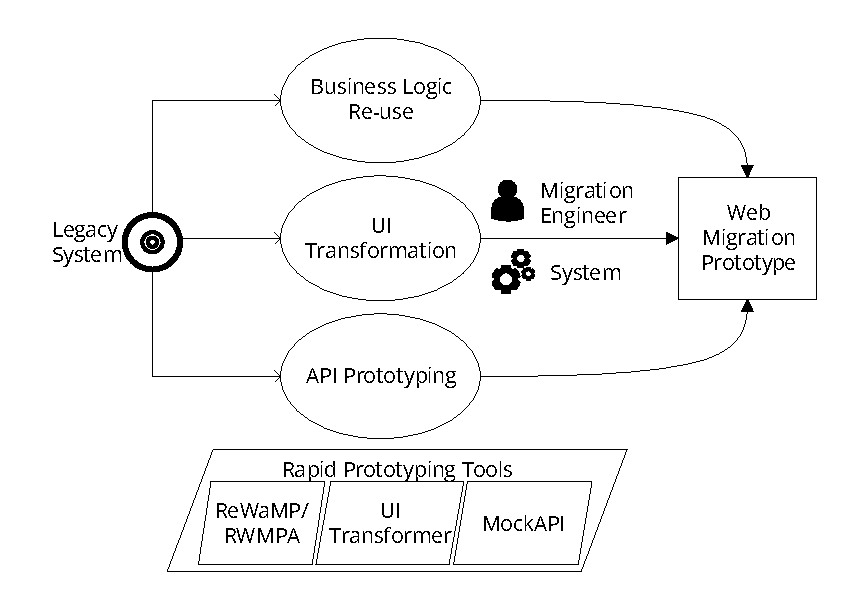
\includegraphics[width=0.98\textwidth]{../figures/solution-rm.pdf}
\caption{AWSM:RM Method Overview}\label{fig:solution-rm}
}
\end{figure}

The \gls{awsm} Risk Management Method (AWSM:RM) shown in \cref{fig:solution-rm} provides a solution for \cref{ro:2} by specifying techniques to demonstrate desirability and feasibility of a potential \glslink{web}{Web}-based version of the \gls{Legacy System}.
AWSM:RM addresses the functional aspect of desirability and feasibility demonstration as well as the non-functional constraint of limited resources and expertise of \cref{ro:2}.
The method transforms existing software \glspl{artifact} defined in the conceptual model for a \gls{Legacy System} specified in \cref{sec:formalisms} into a running \glslink{web}{Web}-based prototype.
AWSM:RM solves \cref{ro:2} through
\begin{itemize}
\item a process for rapid, semi-automatic creation of \glspl{web migration prototype}, supported by API Prototyping
\item a technique for business logic reuse in \glspl{web migration prototype} based on \glslink{wasm}{WebAssembly}
\item a technique for automatic \gls{Transformation} of legacy user interface to \glslink{web}{Web}-based user interface prototypes
\end{itemize}

\par\smallskip
Unlike existing \gls{risk management} methods in the early stages of \gls{Web Migration}, AWSM:RM allows to create a concrete and tangible contribution to the \gls{business case} that serves as a means of communication for stakeholders to support decision making.
To achieve this, \gls{awsm} introduces the novel idea of \gls{Rapid Web Migration Prototyping} \autocite{Heil2018ReWaMP} by transferring the \emph{\gls{Rapid Prototyping} paradigm} \autocite{Gordon1995RapidPrototyping} from \gls{Forward Engineering} into the \gls{Web Migration} domain.
AWSM:RM defines a process for rapidly creating \gls{Web Migration} prototypes based on the \gls{Legacy System} \glspl{artifact}.

To address the constraint of limited resources and \gls{Web Engineering} expertise in \cref{ro:2}, AWSM:RE leverages the WebAssembly \gls{w3c} standard \autocite{W3C2018WebAssembly} to allow reuse of existing business logic.
In this way, the semi-automated prototyping technique can be applied by  \gls{isv}'s existing staff with experience in the legacy technology.
Additional guidance is provided to reduce the required \gls{Web Migration} expertise.

For creating a \glslink{web}{Web}-based user interface prototype, AWSM:RM allows to automatically transform legacy user interfaces based on an evolutionary optimization algorithm.
It addresses the challenge of mapping pixel-based legacy desktop user interface layouts to responsive grid layouts commonly used in \glspl{Web Application}.
AWSM:RM is described in detail in \cref{sec:awsm-rm}.

\vspace{-10pt}
\hypertarget{awsm-customer-impact-control-method}{%
\subsection{AWSM Customer Impact Control Method}\label{awsm-customer-impact-control-method}}
\vspace{10pt}

\begin{figure}[h!]
\hypertarget{fig:solution-ci}{%
\centering
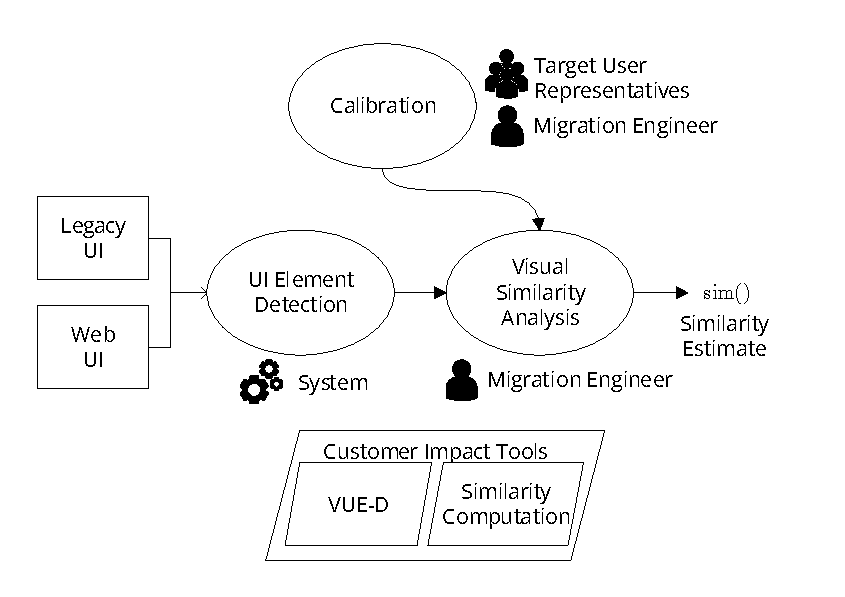
\includegraphics[width=0.98\textwidth]{../figures/solution-ci.pdf}
\caption{AWSM:CI Method Overview}\label{fig:solution-ci}
}
\end{figure}

The \gls{awsm} Customer Impact Control Method (AWSM:CI) shown in \cref{fig:solution-ci} provides a solution for \cref{ro:3} by specifying techniques to control the impact of \gls{Web Migration} on the user bases of existing customers. % with limited resources and lack of \gls{Web Engineering} expertise.
AWSM:RM addresses the functional aspect of customer impact control as well as the non-functional constraint of limited resources and expertise of \cref{ro:3}.
Based on the conceptual model of \glslink{Legacy System}{legacy} user interfaces specified in \cref{sec:formalisms}, AWSM:CI defines a visual similarity measure that allows determining and thus control the degree of visible changes introduced into the user interface through \gls{Web Migration}.
AWSM:CI solves \cref{ro:3} through
\begin{itemize}
\item a model for analysis of visual similarity between legacy \gls{Desktop Application} user interfaces and migrated \glslink{web}{Web}-based user interfaces
\item a process for calibrating the similarity model with a limited number of users
\item a technique for automatically detecting user interface elements
\end{itemize}

\par\smallskip
Unlike existing \gls{Web Migration} approaches, AWSM:CI explicitly addresses the concern of maintaining a similar look and feel between legacy and migrated system by defining a visual \gls{ui} analysis model.
This model allows to compute a measure of visual similarity based on automatically detectable visual aspects to resemble human perception of user interfaces.

To address the constraint of limited resources and \gls{Web Engineering} expertise in \cref{ro:3}, AWSM:CI avoids extensive empirical data collection with large numbers of test subjects and user interface combinations.
Instead, it specifies a process for calibrating the similarity model to the characteristics of the target user group with only a limited number of representatives and specifically designed test samples.
In this way, the similarity measurement can be calibrated with limited effort in initial migration phases and then automatically applied for large numbers of user interfaces created throughout \gls{Web Migration}.

The challenge lies in calculating object-dependent measures due to the heterogeneity of technologies and corresponding description formats for user interface elements.
While existing automatic analysis methods for \gls{web} user interfaces rely on \gls{dom}\footnote{Document Object Model, cf.~\autocite{W3C2015DOM}} analysis, the AWSM:CI similarity measure is applicable to both \glslink{Legacy System}{legacy} and \gls{web} user interfaces \autocite{Heil2016Similarity}.
To achieve this, AWSM:CI contributes to the novel field of research on visual analysis of user interfaces employing deep learning to automatically detect elements of the user interface, enabling calculation of derivative object-dependent measures.
%Following principle \cref{p:1}, analysis results are made available using JSON.
AWSM:CI is described in \cref{sec:awsm-ci}.

\vspace{-13pt}
\hypertarget{sec:platform}{%
\section{Tools}\label{sec:platform}}
\vspace{12pt}

The \gls{awsm} Toolsuite provides support tools for the methods of the \gls{awsm} Methodology addressing the overarching goal and research objectives.
It represents a \glslink{web}{Web}-based \gls{Reverse Engineering} and \gls{Web Migration} management system to support management and \gls{migrationengineer} stakeholders, providing 
\begin{itemize}
\item a decision support system for Web Migration strategy formation,
\item a migration monitoring and management dashboard with software quality visualizations,
\item a \glslink{Legacy System}{legacy} knowledge repository with a query endpoint,
\item a concept-assignment-based \gls{Reverse Engineering} tool,
\item a set of tools for crowd-based knowledge discovery,
\item a business logic \gls{Transformation} tool for \gls{Rapid Web Migration Prototyping},
\item a tool for generation of RESTful APIs from legacy system screenshots,
\item a tool for \gls{Transformation} of legacy user interfaces to \glslink{web}{Web}-based user interfaces,
\item a process guidance and orchestration tool for \gls{Rapid Web Migration Prototyping}, 
\item a measurement tool for customer impact through \gls{Web Migration}, 
\item a visual user interface element detector.
\end{itemize}

The following subsections provide an overview of these \gls{awsm} Tools.
Several tools are grouped together by their relationship to each of the three research objectives and corresponding \gls{awsm} Methods.

\vspace{-15pt}
\hypertarget{sec:s2dcs}{%
\subsection[AWSM Strategy Selection Decision Support Syst.]{AWSM Strategy Selection Decision Support System}\label{sec:s2dcs}}
\vspace{15pt}

The \gls{s2dcs} addresses the overarching goal \cref{og} by solving the problem of selecting a global migration strategy tailored to the situation of the \gls{isv} at the initiation of \gls{Web Migration}.
Within that \gls{Reengineering} or \gls{Transformation} strategy, the \gls{awsm} Methodology provides solutions addressing the identified gaps in current \gls{Web Migration} approaches.
The migration strategy determines the phases in \cref{fig:methods-techniques-tools} and thus the outer context in which the \gls{awsm} Methods and Tools are applied.
Selecting a suitable approach for the specific situation is a challenge for \glspl{isv} due to the wide range of approaches, as shown in \cref{sec:approaches}.
The \gls{s2dcs} tool is a decision support system based on the results of our systematic mapping study \autocite{Heil2017Survey}, which identified and evaluated 122 primary studies, comprising not only academic publications but also existing software tools.
%It supports \glspl{isv} to either employ the approach that suits best to their specific \gls{Web Migration} problem or build their own composite strategy based on the information provided from a set of appropriate approaches.
To address the constraints of \cref{og}, \gls{s2dcs} represents a \emph{faceted search} interface \autocite{Tunkelang2009FacetedSearch} so that \glspl{isv} with limited resources and lack of \gls{Web Migration} expertise are supported in formation of their migration strategy by being given easy access to a wide range of information that would have otherwise required extensive time, effort and expertise to accumulate.

Supporting non-technical Management stakeholders, as described in \cref{sec:problem-analysis-results}, the faceted search is realized as a guided dialogue interaction, as shown in \cref{fig:s2dcs}.
\begin{figure}[h!]
\hypertarget{fig:s2dcs}{%
\centering
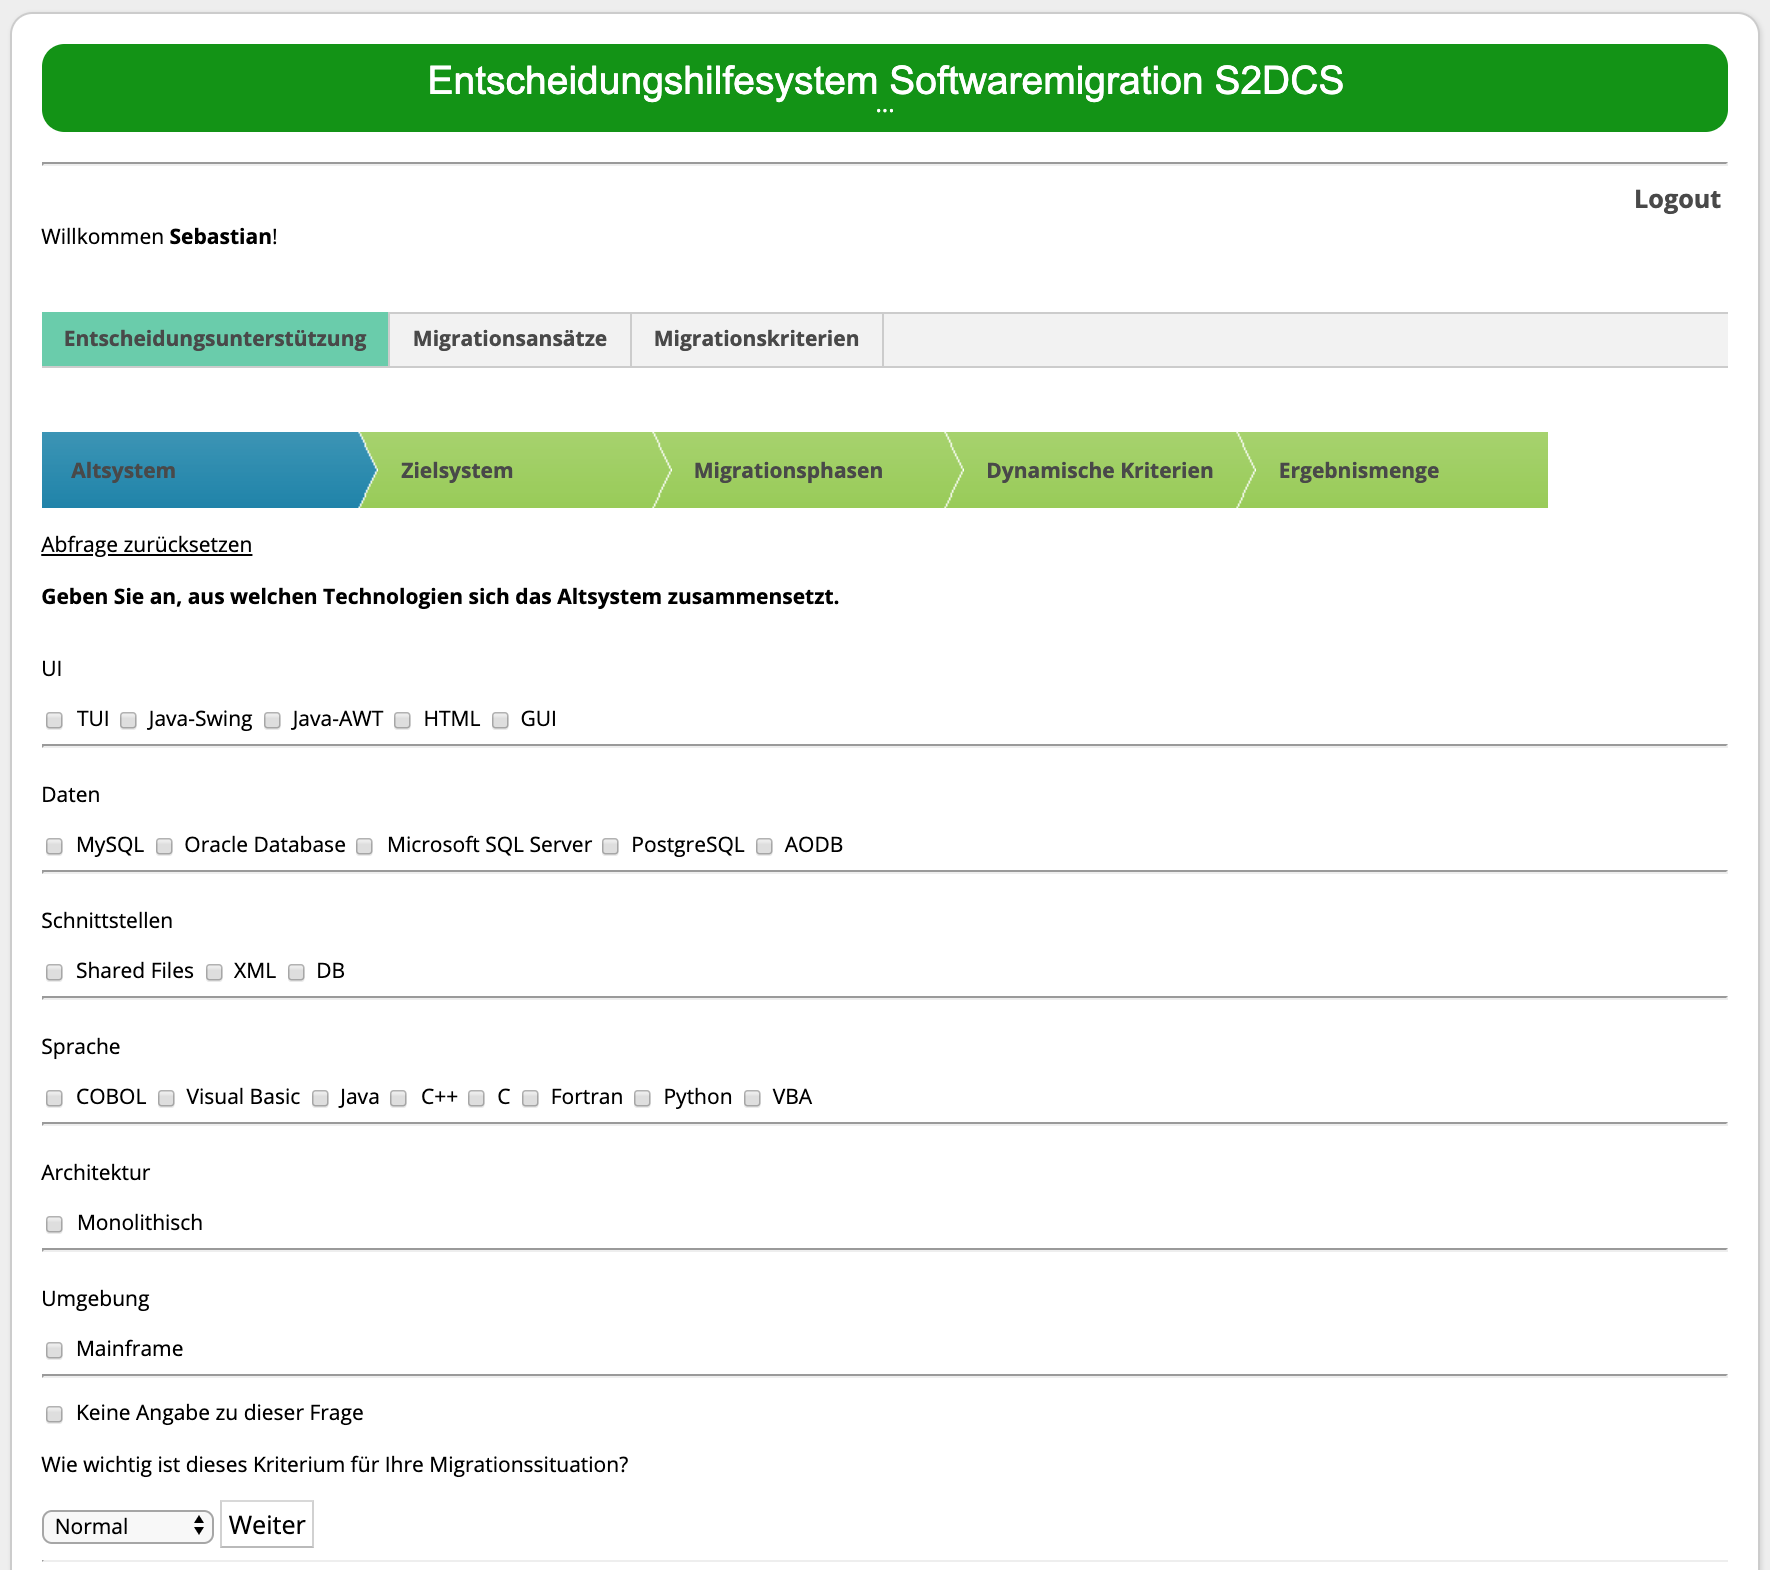
\includegraphics[width=0.98\textwidth]{../figures/screenshots/s2dcs-query-new.png}
\caption[S2DCS Entry of Migration Situation ]{S2DCS Entry of Migration Situation View, First Step in Faceted Search: Legacy System Characteristics (German)}\label{fig:s2dcs}
}
\end{figure}
The \gls{s2dcs} user answers a set of questions dynamically created from the available criteria and values in order to specify his \gls{Web Migration} scenario, i.e.~the as-is and to-be state and constraints.
The answers form the search facets that define the query on the knowledge base.
To construct the result set, candidate approaches are ranked according to their compliance with the query.
The criteria for selecting approaches are defined by \glslink{target system}{target} and \gls{source system} characteristics (e.g.~architectures, technologies), supported migration phases and dynamic criteria depending on the selection of the other criteria.

The user is shown a ranked list of approaches and tools matching  his search criteria, as displayed in \cref{fig:s2dcs-results} and can review details and access information about authors, year of creation, a brief description, the main project or publication URL, complimentary linked resources such as reports and case studies, as well as available evidence of successful application, industrial relevance and tool support.
The \gls{s2dcs} is designed to allow the selection criteria, catalog data, and the dataset of its \knowledgebase to be extended through configuration to allow updating the \gls{Web Migration} approaches.

\vspace{-10pt}
\hypertarget{sec:tools.annotationplatform}{%
\subsection{AWSM Annotation Platform}\label{sec:tools.annotationplatform}}
\vspace{10pt}

The Annotation Platform implements knowledge discovery and management tools for the \gls{awsm} Reverse Engineering Method solving \cref{ro:1} and a support system for controlling \gls{Web Migration} execution.
To support the techniques of AWSM:RE, \gls{migrationengineer} stakeholders can use the Annotation Platform to visualize  software quality aspects of the legacy system code base and to conduct concept-assignment-based \gls{Reverse Engineering} manually, using existing tools for automated \gls{Reverse Engineering} or applying the novel AWSM:RE crowdsourced \gls{Reverse Engineering} approach.
\Cref{fig:ap-dashboard} shows a screenshot of the dashboard view of the Annotation Platform, providing a starting page to access its functionality.
\begin{figure}[h!]
\hypertarget{fig:ap-dashboard}{%
\centering
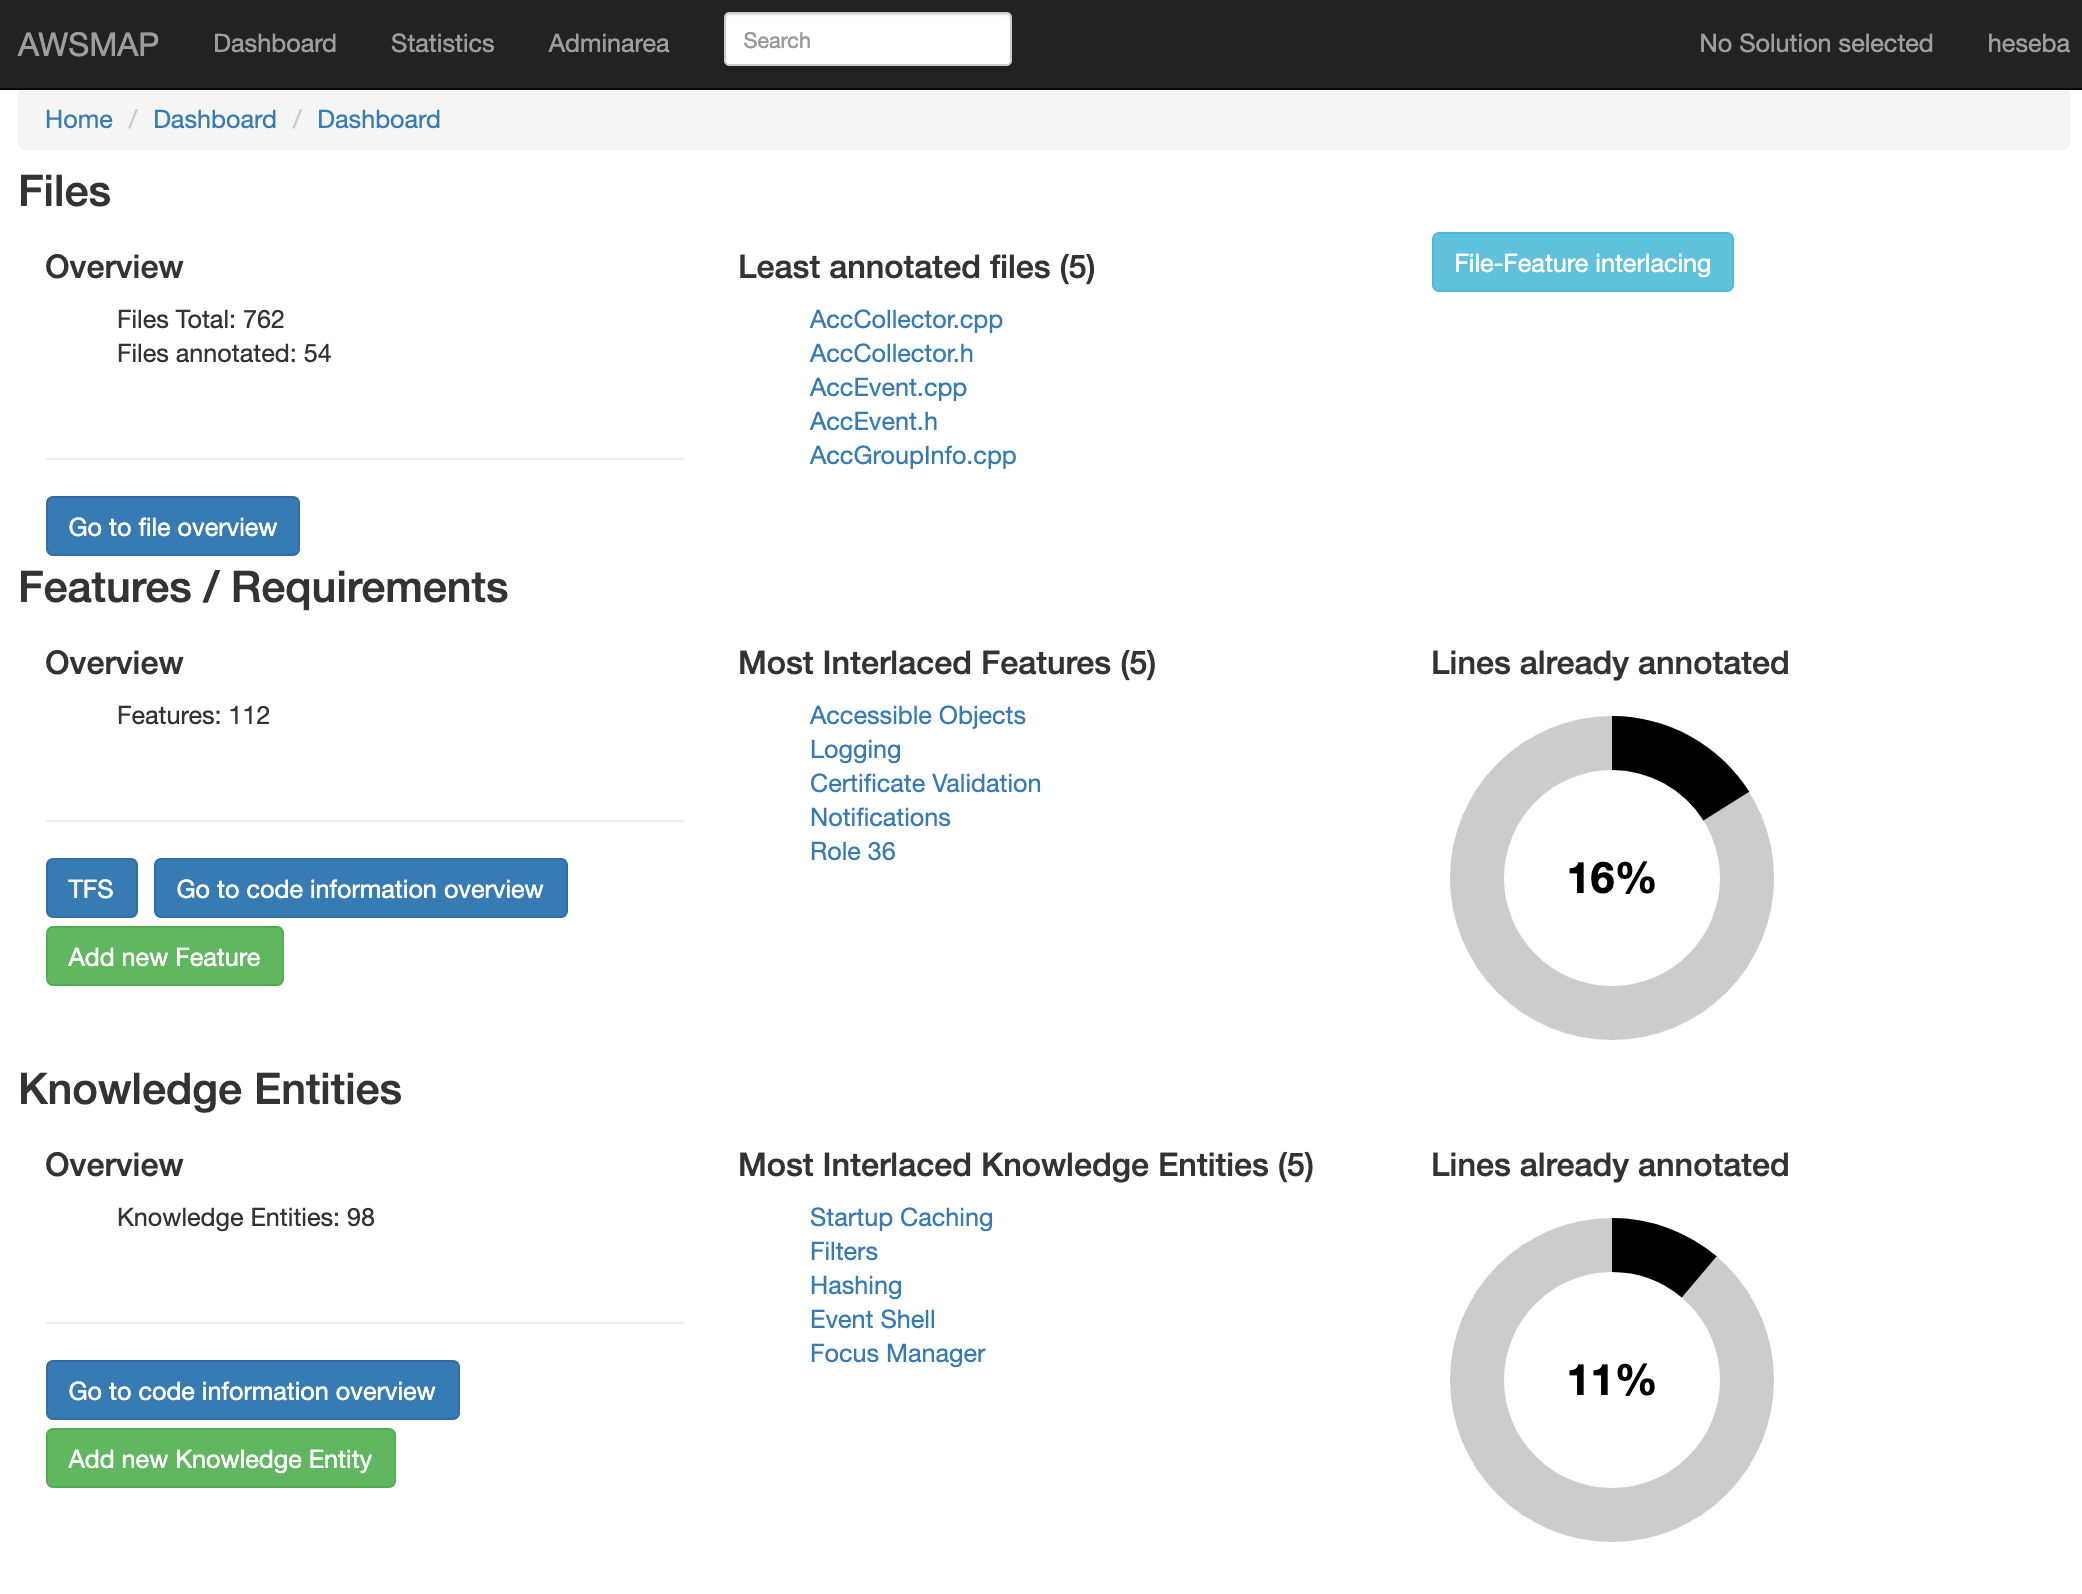
\includegraphics[width=0.98\textwidth]{../figures/screenshots/ap-dashboard-2.png}
\caption{Annotation Platform Dashboard}\label{fig:ap-dashboard}
}
\end{figure}
The tools for crowd-based knowledge discovery implement AWSM:RE techniques for the technical challenges of automatic creation and deployment of micro tasks for crowdworkers, controlling disclosure of legacy source code, and aggregation and quality control of crowdworker results.
These functionalities represent solutions for the identification activity of \cref{ro:1}.
The knowledge management activity of \cref{ro:1} is addressed by its \glslink{web}{Web}-based navigable \glslink{Legacy System}{legacy} knowledge repository for human stakeholders and its standards-based query endpoint for system actors and integration with other \gls{Web Migration} tools. 
The \gls{Web Migration} control part of the Annotation Platform provides a migration monitoring and management dashboard to allow management stakeholders to start and prioritize migration activities and monitor migration progress throughout the execution.
To achieve good integration into ongoing development activities as per requirement \cref{c:4} Agile, the \gls{awsm} Annotation Platform integrates with the existing tools landscape of \glspl{isv}.
For management stakeholders, the Annotation Platform integrates with software project management platforms.
This allows to feed migration-related tasks identified using the Annotation Platform into the backlogs and planning of ongoing development.
For \gls{migrationengineer} stakeholders, the Annotation Platform integrates with integrated development environments (\glspl{ide}).
This allows to conduct \gls{Reverse Engineering} tasks for \gls{Web Migration} during ongoing development activities, leveraging the existing mental models and program comprehension of developers applying changes to the \glslink{Legacy System}{legacy} source code.
The tools which constitute the \gls{awsm} Annotation Platform to address research objective \cref{ro:1} are described in \cref{sec:awsm-re} together with the AWSM:RE method which they support.

\vspace{-10pt}
\hypertarget{sec:tools.rewamp}{%
\subsection{AWSM Rapid Web Migration Prototyping Tools}\label{sec:tools.rewamp}}
\vspace{10pt}

The ReWaMP/RWMPA, MockAPI and UI Transformer tools implement techniques of the \gls{awsm} Risk Management Method addressing \cref{ro:2}.
They realize tool support for the \gls{awsm}'s novel \gls{Rapid Web Migration Prototyping} concept, allowing \glspl{migrationengineer} to quickly create running \glslink{web}{Web}-based prototypes of the \gls{Legacy System} through automatic \gls{Transformation} and process guidance.

ReWaMP leverages \gls{wasm} to implement a reuse based \gls{Transformation} of \glslink{Legacy System}{legacy} business logic.
This allows quick creation of \gls{Web Migration} prototypes through reuse of parts of the \glslink{Legacy System}{legacy} code base and making use of the expertise of existing staff in the \glslink{Legacy System}{legacy} technology.
The technical challenge addressed by ReWaMP lies in achieving a high degree of reuse of  \glslink{Legacy System}{legacy} code and limiting required adaptions in particular for dependency management.
MockAPI supports rapid creation of RESTful API backends through annotation of screenshots of the \glslink{Legacy System}{legacy} user interfaces.
This allows automatic creation of a prototypical \glslink{web}{Web}-based API for \gls{Web Migration} prototypes without specific \gls{Web Engineering} expertise, only requiring identification of the main domain entities represented in \glslink{Legacy System}{legacy} user interfaces.
The technical challenge addressed by MockAPI lies in \gls{Transformation} from a light-weight domain-specific annotation language into a running RESTful API endpoint.
UI Transformer creates \glslink{web}{Web}-based responsive grid layouts from pixel-based \glslink{Legacy System}{legacy} user interfaces.
This allows to automatically generate running \glslink{web}{Web}-based frontend prototypes without \gls{Web Engineering} expertise.
The technical challenge addressed by UI Transformer lies in mapping between the two different layout paradigms of pixel-based and responsive grid while maintaining a sufficient level of visual similarity.
The RWMPA tool guides \glspl{migrationengineer} through the process of \gls{Rapid Web Migration Prototyping}, providing descriptions and plugin-based extensible tool support for each necessary activity, orchestrating the tools and aggregating and forwarding the intermediate results.
The technical challenge addressed by RWMPA lies in providing suitable guidance and tool support to enable \glspl{migrationengineer} without extensive migration expertise to apply the AWSM:RM method and reduce the amount of manual interventions required.
\Cref{fig:rwmpa-select} shows the view selection dialog of the RWMPA assistance system, allowing to choose the source material from existing \legacy \glspl{artifact} to start assisted prototyping. 

Together, the ReWaMP/RWMPA, MockAPI and UI Transformer tools enable rapid creation of \gls{Web Migration} prototypes for risk management \gls{Web Migration} phases in support of the AWSM:RM method solving \cref{ro:2}.
They represent the first concrete implementation of applying the \gls{Rapid Prototyping} paradigm to the \gls{Web Migration} domain for both frontend and backend.
The \gls{awsm} \gls{Rapid Web Migration Prototyping} Tools to address research objective \cref{ro:2} are described in \cref{sec:awsm-rm} together with the AWSM:RM method which they support.
\begin{figure}[h!]
\hypertarget{fig:rwmpa-select}{%
\centering
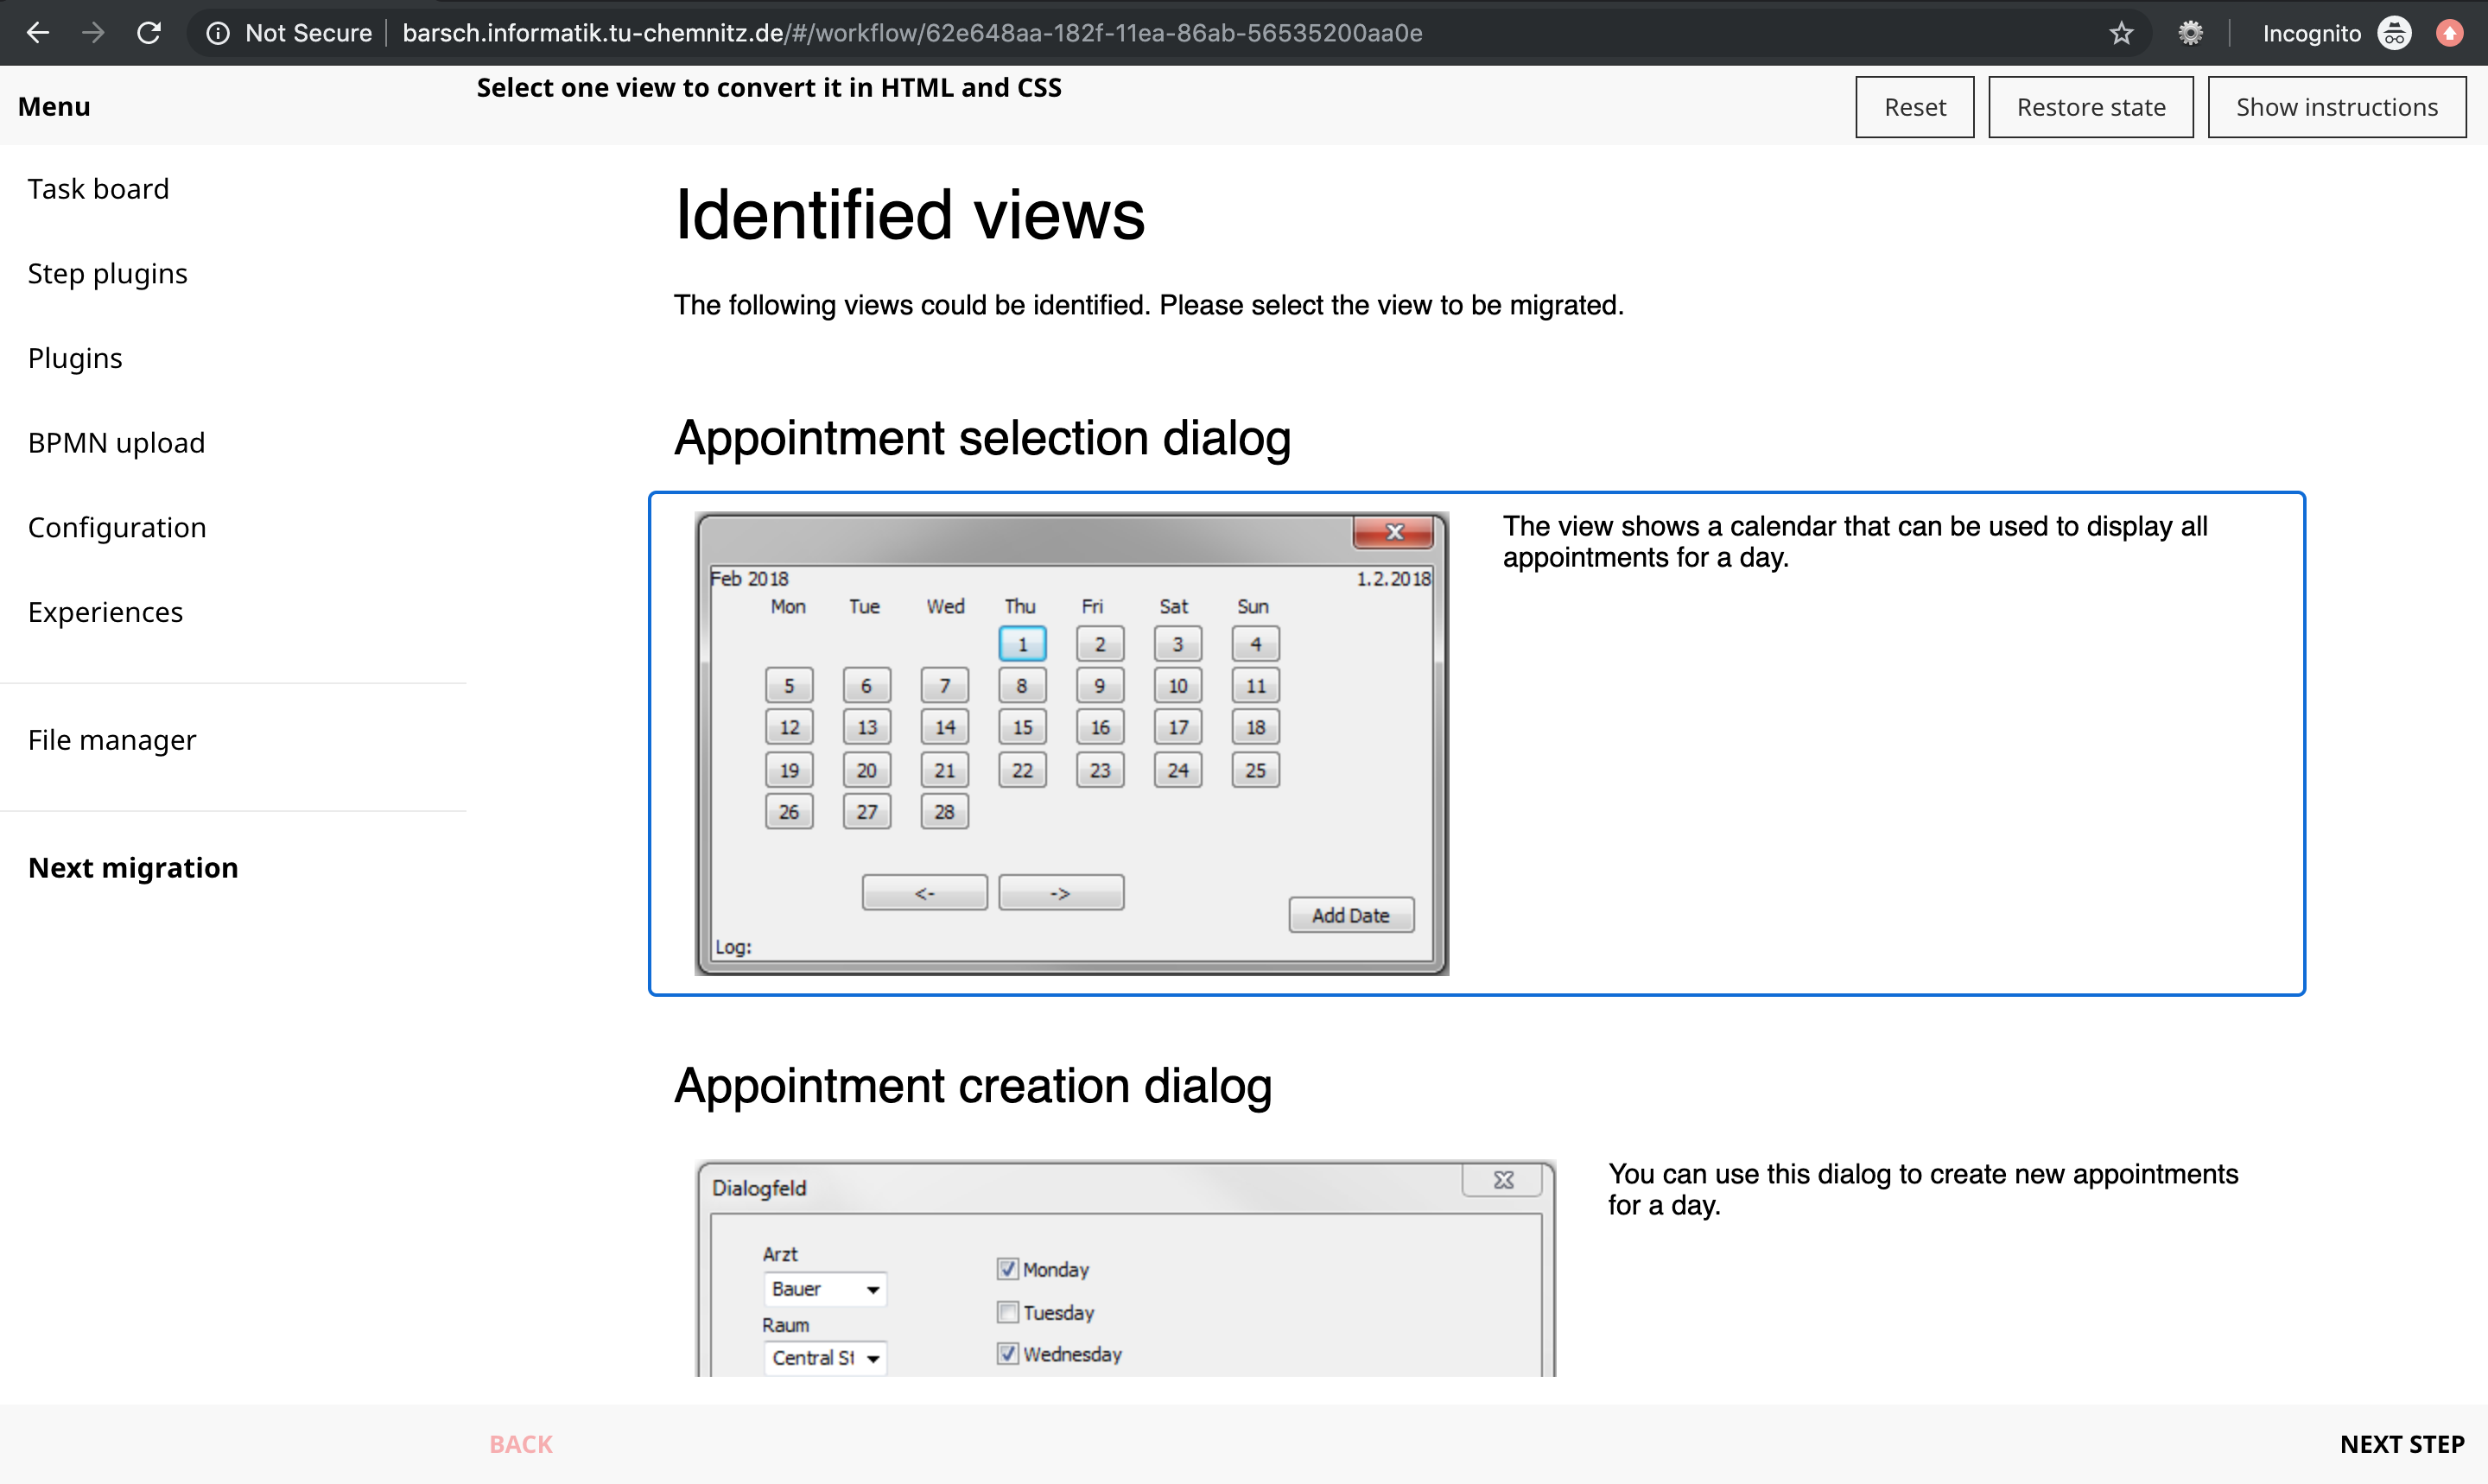
\includegraphics[width=0.98\textwidth]{../figures/screenshots/rwmpa-select.png}
\caption{RWMPA View Selection}\label{fig:rwmpa-select}
}
\end{figure}

\vspace{-20pt}
\hypertarget{sec:tools.ci}{%
\subsection{AWSM Customer Impact Tools}\label{sec:tools.ci}}
\vspace{10pt}

The Customer Impact Tools realize techniques of the \gls{awsm} Customer Impact Control Method addressing \cref{ro:3}.
They provide tool support for quantifying the similarity between \glslink{Legacy System}{legacy} non-\glslink{web}{Web} user interfaces before, and \glslink{web}{Web}-based user interfaces after migration to control the impact of visible layout changes through \gls{Web Migration}.

To address the limited resources constraint of \cref{ro:3}, the Customer Impact Tools allow the computation of a similarity function.
Instead of the high effort required for pair-wise empirical comparisons of user interfaces, this similarity function works as an approximation for perceived user interface similarity.
It is based on a vector-space model of distances in several user interface similarity dimensions, each of which can be computed without manual intervention from objective measures on screenshots of user interfaces.
This allows measuring the similarity between existing \glslink{Legacy System}{legacy} user interfaces and newly created \glslink{web}{Web}-based user interfaces using computable measures instead of time-consuming and expensive empirical experimentation, providing a basis for comparing alternatives and defining a step-wise transition to the target layout with controlled impact in each step.
Here, the technical challenge addressed by the  VUE-D tool lies in calculating object-dependent measures such as variations in user interface element order across non-\glslink{web}{Web} migration source and \glslink{web}{Web}-based migration \gls{target system}.
VUE-D provides a solution for automatically detecting user interface elements in both \glslink{Legacy System}{legacy} and \glslink{web}{Web}-based user interfaces independent of the heterogeneous technologies and description formats.
\Cref{fig:vue-d} shows a \web user interface analyzed by VUE-D, combining shape detection (in red) with OCR (in green) results.
\begin{figure}[h!]
\hypertarget{fig:vue-d}{%
\centering
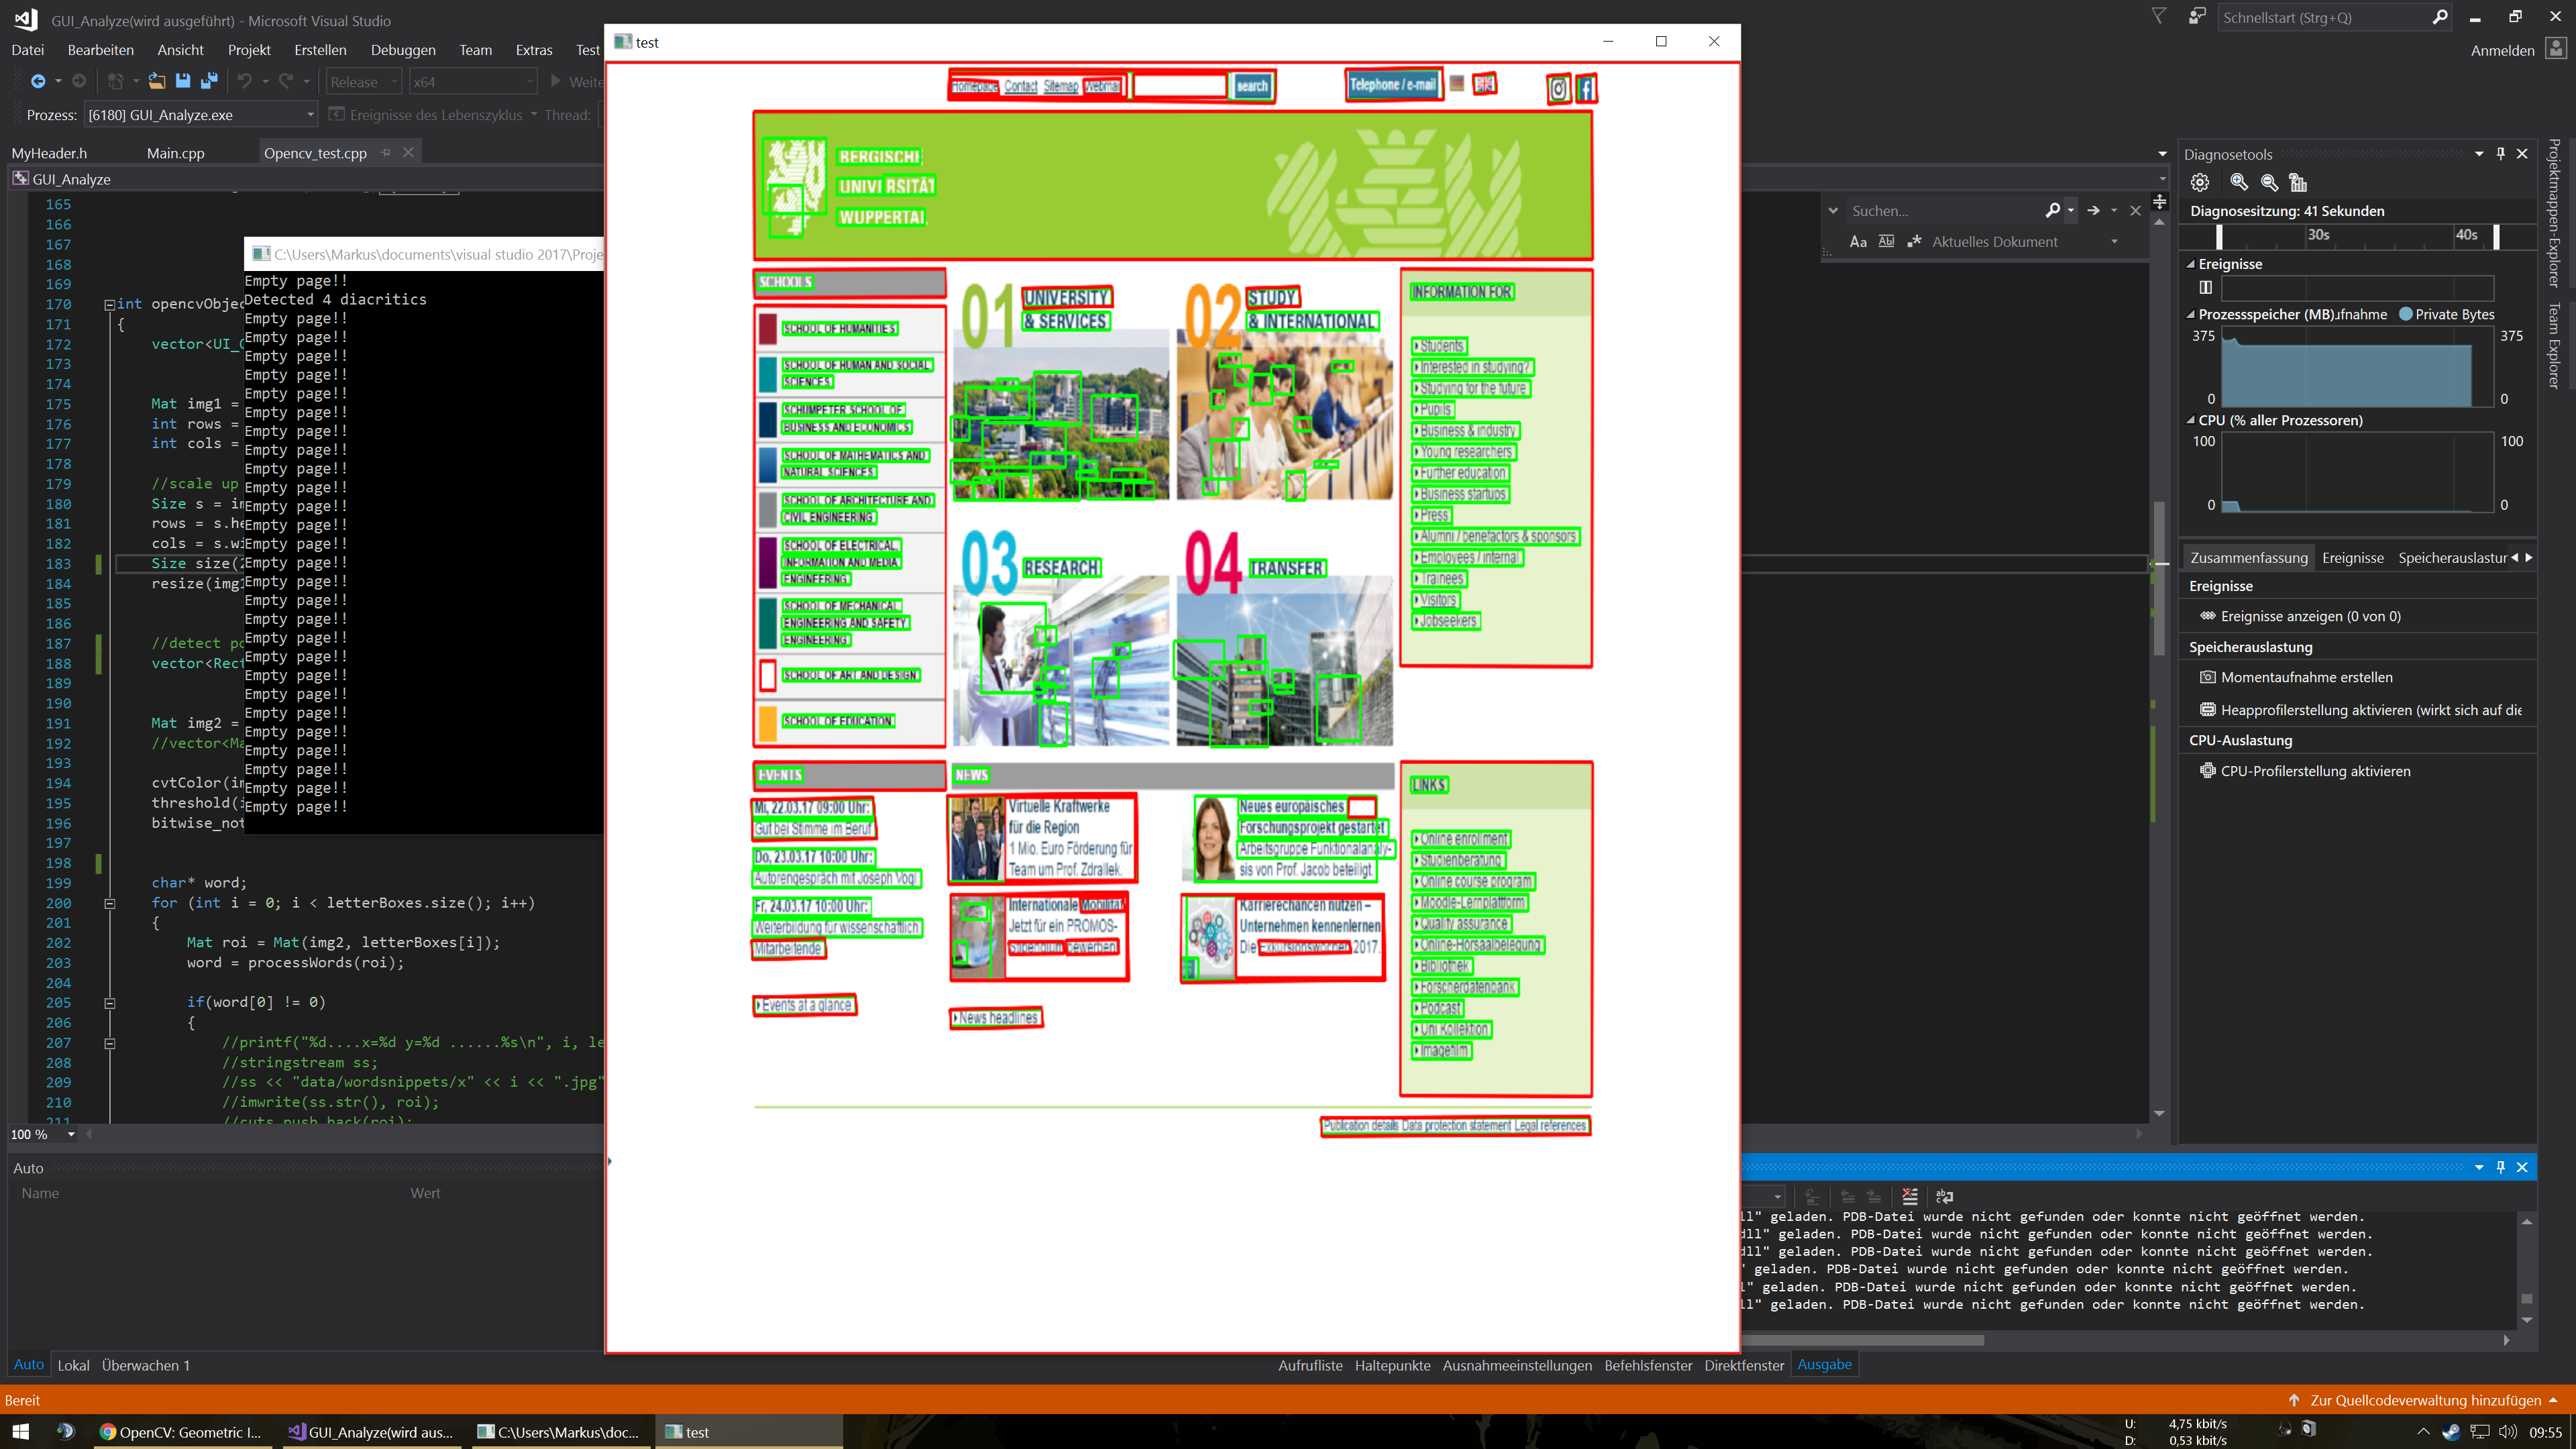
\includegraphics[width=0.98\textwidth]{../figures/screenshots/UI-Element-Recognition.png}
\caption{VUE-D UI Element Detection}\label{fig:vue-d}
}
\end{figure}
Unlike existing approaches which require specific textual representations of the user interface like \gls{dom}, it works on purely visual input data by applying computer vision techniques for locating areas of interest and machine learning techniques for classification of user interface element types.
This allows to operate independent of specific \glslink{Legacy System}{legacy} and \glslink{web}{Web}-based user interface technologies and to restrict the input to visible characteristics that are the basis for human perception.
The \gls{awsm} Customer Impact Tools to address research objective \cref{ro:3} are described in \cref{sec:awsm-ci} together with the AWSM:CI method which they support.

\vspace{-20pt}
\hypertarget{principles}{%
\section{Principles}\label{principles}}
\vspace{5pt}

The \gls{awsm} Methodology and Toolsuite are built on four principles.
These principles provide solutions to address the shortcomings in the state of the art of \gls{Web Migration} identified in \cref{sec:sota.shortcomings} that are cross-cutting non-functional concerns for each of the three research objectives.
Therefore, they drive design decisions of all methods and tools in the \gls{awsm} Methodology and Toolsuite.
The following \gls{awsm} Principles formulate four top-level design decisions of \gls{awsm} and their rationale:

\vspace{-10pt}
\begin{thesisprinciple}{Open \gls{web} Standards}{p:1}
To address the problem of technology-specificity of \gls{Web Migration} approaches limiting their applicability and inhibiting interoperability, this principle advocates using and extending open \gls{web} standards in the \gls{awsm} Methodology and Toolsuite.
The use of standards is widely accepted in software engineering and \gls{Web Engineering}.
For \gls{Web Migration}, using in particular \gls{w3c} specifications and \gls{omg} migration standards allows interoperability with existing methods and tools and provides contributions that can easily be used and enhanced by future research (cf.~OpenStand Principles\footnote{\url{https://open-stand.org/about-us/principles/} Retrieved: 6.12.2019}).
This especially applies to underlying data models, provided interfaces and technologies used in \gls{awsm}.
\end{thesisprinciple}

\vspace{-10pt}
\begin{thesisprinciple}{Methodology over Process}{p:2}
To address the problem of a wide range of existing \gls{Web Migration} approaches with individual process models on the one hand, and their shortcomings with regard to \gls{Web Migration} initiation for \glspl{isv} with limited resources and lack of \gls{Web Engineering} expertise on the other hand, \gls{awsm} aims at providing a \emph{methodology} that addresses these shortcomings.
This principle advocates an integration with existing \gls{Web Migration} \gls{Reengineering} and \gls{Transformation} process models to prefer reuse over re-definition of a new \gls{Web Migration} process model.
Therefore, \gls{awsm} Methods are designed for embedding within the context of other \gls{Web Migration} approaches, as depicted in \cref{fig:methods-techniques-tools}.
%Therefore, \gls{awsm} Methods define mappings for extension of the most relevant \gls{Web Migration} approaches such as REMICS, ARTIST or UWA/UWAT+.
\end{thesisprinciple}

%\pagebreak
%\vspace{-10pt}
\begin{thesisprinciple}{Model-Driven Agnosticism}{p:3}
To address the limited applicability of \gls{Web Migration} approaches due to the divide of the current \gls{Web Migration} landscape on the use of \gls{mde}, the \gls{awsm} Methodology and Toolsuite are agnostic to Model-Driven adoption.
This is required, since half of the approaches in \cref{sec:approaches}  employs \gls{mde} in some form, and half of the approaches does not.
Likewise, \gls{mde} practices are employed in varying degrees in forward \gls{Web Engineering} \autocite{Moreno2008MDWE}.
This principle advocates compatibility with Non-Model-Driven \gls{Web Migration} approaches as well as with \gls{Web Migration} approaches at different degrees of Model-Driven adoption.
In particular \gls{Reverse Engineering}, which forms the basis of \gls{Reengineering} and \gls{Transformation}, is laid out agnostic but adaptable to concrete Model-Driven or Non-Model-Driven methods in \gls{awsm} to allow interoperability with a wide range of existing \gls{Web Migration} approaches.
\end{thesisprinciple}

\vspace{-10pt}
\begin{thesisprinciple}{Rapid Prototyping Paradigm}{p:4}
To address the problem of a lack of demonstration of desirability for decision making in initial \gls{Web Migration} phases, this principle advocates applying the \gls{Rapid Prototyping} paradigm to the \gls{Web Migration} domain.
\gls{Prototyping} is an established means of improving quality in forward software engineering \autocite{Wallmueller2001SoftwareQuality}.
The \gls{Rapid Prototyping} paradigm \autocite{Gordon1995RapidPrototyping} with its dedicated focus on quick and cheap creation of tangible means of communication of envisioned software for all involved stakeholders \autocite{Alavi1984} is particularly common in the context of Agile Development \autocite{Abrahamsson2002Agile} and Human-Centered Design \autocite{HCD2015}.
Thus, the \gls{awsm} Methodology and Toolsuite favor the creation of prototypes as concrete, tangible means of communication to demonstrate desirability of a \glslink{web}{Web}-based version of the migrated \gls{Legacy System} over theoretical and general argumentation and narrowly focused technical feasibility studies.
\end{thesisprinciple}

%\pagebreak
\vspace{-15pt}
\hypertarget{sec:formalisms}{%
\section{Formalisms}\label{sec:formalisms}}
\vspace{10pt}

The \gls{awsm} Methodology provides solutions for the three research objectives.
These solutions are based on a common theoretical basis, the \gls{awsm} Formalsisms specified in this section.
The formalisms define basic \emph{conceptual models} independent of their concrete implementation in the \gls{awsm} Toolsuite.
%The conceptual architecture of the \gls{awsm} Toolsuite is discussed in \cref{sec:platform}.
\gls{awsm} defines three formalisms:
\begin{itemize}
\item Legacy System
\item Source Code Knowledge Model
\item Legacy User Interface
\end{itemize}
The \gls{Legacy System} formalisms defines a \gls{Legacy System} in terms of its \emph{software \glspl{artifact}} \autocite{OMG2016KDM}, i.e.~of physical resources that are available as inputs for analysis and \gls{Transformation} activities described in the methods of the \gls{awsm} methodology.
The Source Code Knowledge Model formalism defines the knowledge contained in a \gls{Legacy System} in terms of relevant \emph{software assets} \autocite{OMG2016KDM} that are represented through the \glspl{artifact} but not necessarily existing in explicit forms.
The Legacy User Interface formalism defines a uniform description of user interfaces and their conceptual components to support \gls{awsm}'s focus on maintaining user interface consistency across legacy and target technologies.

As a design decision reasoned in principle \cref{p:1}, AWSM Formalisms extend \gls{omg}'s Knowledge Discovery Meta-Model specification.
On the one hand, this allows \gls{awsm} to reuse the semantics specified in \gls{kdm} and avoid lengthy descriptions and re-definitions.
On the other hand, \gls{kdm}'s technical focus on file-based knowledge representation is insufficient for the \gls{awsm} Methodology.
Therefore, \gls{awsm} makes use of \gls{kdm}'s extension mechanism to effectively use only parts necessary \autocite{OMG2016KDM} for the \gls{awsm} Methods and adds the required missing semantics.
For brevity, when referring to \gls{kdm} in the following description of formalisms, these references are to be considered as a reference to \gls{kdm} version 1.4 of September 2016 \autocite{OMG2016KDM}.

\vspace{-18pt}
\hypertarget{sec:formalisms.ls}{%
\subsection{Legacy System}\label{sec:formalisms.ls}}
\vspace{4pt}

The \gls{Legacy System} formalism specifies the conceptual model of the central object of investigation of this thesis and is used to describe the source material of all \gls{awsm} Methods and Tools.
%A \gls{Legacy System} is the basis for any \gls{Web Migration} and the central object of investigation of this thesis, serving as the starting point for the three \gls{awsm} Methods.
\gls{kdm} \autocite{OMG2016KDM} provides a comprehensive \emph{\gls{metamodel}} for describing \glspl{Legacy System}.
\gls{awsm}'s conceptual model of a \gls{Legacy System} is based on \gls{kdm} concepts that provide the common foundation for the structure of \glspl{Legacy System} in the context of the \gls{awsm} Methodology.
%In particular, the \emph{inventory model} of the \gls{kdm} \emph{source package}, the \emph{platform package} and the \emph{\gls{ui} package} are relevant for \gls{awsm}.
\vspace{-15pt}
\begin{thesisdefinition}{Legacy System Formalism}{def:ls-formalism}
In \gls{awsm}, a \gls{Legacy System} \(\mathfrak{L}\) is a 6-tuple of a legacy codebase, a set of dependencies, a dependency matrix, a set of executables, a set of persistent data and a set of legacy user interfaces:
\begin{equation}\mathfrak{L} = (B, Dep, \underline D,  E, D, U)\label{eq:legacy-system}\end{equation}
\end{thesisdefinition}

\vspace{-5pt}
\textbf{Legacy codebase \(B\)} consists of a set of source code files (\gls{kdm}: SourceFile), configuration files (\gls{kdm}: \emph{ConfigFile}) and other textual documents (\gls{kdm}: \emph{Document}).

\textbf{Dependencies \(Dep\)} represent external dependencies of the \gls{Legacy System} (\gls{kdm}: \emph{LinkableFile}), in particular third-party libraries (\gls{kdm}: \emph{LibraryFile}).

\textbf{Dependency matrix \(\underline D\)} defined as \(\underline D: \{1,\ldots, |B|\} \times \{1,\ldots, |Dep|\} \mapsto [0,1]\) is a binary matrix with \(\underline D_{i,j} = 1 \Longleftrightarrow f_i \in B\) depends on \(dep_j \in Dep\), else \(\underline D_{i,j} = 0\).

\textbf{Executables \(E\)} are the software executables (\gls{kdm}: \emph{ExecutableFile}) of the \gls{Legacy System}.
In some cases, \(B\) or \(E\) can be \(B=E=\emptyset\) \autocite{Binkley2007b}; however, as described in \cref{sec:scenario-code}, we assume availability of source code and executables in this thesis.

\textbf{Persistent data \(D\)} represents data stored or accessed by the \gls{Legacy System}, such as databases or storage files (\gls{kdm}: \emph{FileResource}).

\textbf{User interfaces \(U\)} are the resources that form the user interface (\gls{kdm}: \emph{UIModel}) of the \gls{Legacy System}, consisting of container resources (\gls{kdm}: \emph{UIResource}) like screens.
The elements of \(U\) are not identical to their formal representation in \(B\) (e.g.~\gls{xaml} files, \gls{mfc} resource files), but they are resulting from it and part of the executables in \(E\) from where their visual (i.e.~pixel-based) representation can be retrieved.
The \glslink{Legacy System}{legacy} user interface is described in more detail in \cref{sec:ui-formalism}.

\vspace{-10pt}
\hypertarget{sec:formalisms.sckm}{%
\subsection{Source Code Knowledge Model}\label{sec:formalisms.sckm}}
\vspace{10pt}

To achieve \cref{ro:1}, the risk of losing knowledge through \gls{Web Migration} needs to be addressed by extracting, capturing, and preserving valuable knowledge in the \gls{Legacy System}.
The \gls{sckm} formalism is the part of the \gls{awsm} solution that allows to represent arbitrary knowledge in \glspl{Legacy System}.

%The \gls{sckm} is at the core of the \gls{awsm} Reverse Engineering Method.
%As argued in the introduction, \glspl{Legacy System} contain valuable \emph{knowledge from the problem and solution domain} \autocite{Marcus2004ProblemLocation} that must be preserved throughout migration.

The challenge addressed by the \gls{sckm} is the implicit nature of knowledge in \glslink{Legacy System}{legacy} code bases: similar to \emph{tacit knowledge} in organizations which is
not expressed explicitly but guides human behavior \autocite{Nonaka2008TacitKnowledge}, the knowledge in \glspl{Legacy System} is not explicitly documented but governs how they operate.
Codification is required to make it explicit, which is achieved through \emph{reverse engineering}.
The knowledge reverse-engineered from the \glslink{Legacy System}{legacy} source code through redocumentation and design recovery needs to be represented at different levels of abstraction and stored in a \emph{knowledge base} to feed into subsequent \gls{Reengineering} or \gls{Transformation}.


\gls{omg}'s \gls{kdm} is insufficient for describing implicit knowledge.
%provides a basic model for \glslink{Legacy System}{legacy} source code knowledge above procedure level in the \gls{kdm} specification as described in \cref{sec:adm}.
%Thus it is used as the basis for the \gls{sckm}.
It is focused on redocumentation knowledge, i.e.~equivalent representations of knowledge within the same abstraction level, the implementation level, describing the structure of the \glslink{Legacy System}{legacy} codebase in terms of modules, classes, methods, files.
\gls{kdm} assumes knowledge to reside in dedicated files -- data in data files, configuration in configuration files, etc.
-- whereas knowledge often appears mixed, due to the missing separation of concerns in \glspl{Legacy System}, within the source code.

Therefore, the \gls{sckm} allows the representation of design recovery knowledge, i.e.~knowledge on higher levels of abstraction, free of the assumption of explicit representation while maintaining the connection to its occurrence in structural parts of the source code.
The \gls{sckm} formalism specifies two conceptual models:
\begin{itemize}
\item a unified knowledge model independent of explicit physical representations,
\item a model for linking knowledge to its occurrences within artifacts of the legacy code.
\end{itemize}

\vspace{-15pt}
\subsubsection*{Unified knowledge model} 
In \gls{awsm}, an instance of knowledge \(k\) in the \gls{Legacy System} \(\mathfrak{L}\) is a tuple

\begin{equation}k = (t, r)\label{eq:knowledge}\end{equation}

of type \(t \in T\) and a representation \(r\).
%
%Types
%Migration aims at retaining the functionality of \glspl{Legacy System} in new environments \autocite{Bisbal1999LegacyInformationSystems}, with functionality referring to domain knowledge and business logic \autocite{Wagner2014}.
\gls{awsm} considers two basic varieties of knowledge in \glslink{Legacy System}{legacy} source code:
\begin{itemize}
\item \emph{Features} describe functionality of the \gls{Legacy System} (What) and can be represented as user stories, scenarios, use cases etc.
\item \emph{Domain knowledge} is the knowledge supporting the implementation of features, describing parts of the problem and solution domain of the \gls{Legacy System} (How).
\end{itemize}
Domain knowledge is divided into problem and solution domain knowledge \autocite{Marcus2004ProblemLocation}.
In \gls{sckm}, problem domain knowledge comprises business processes and business rules.
Solution domain knowledge comprises presentation, persistence, algorithms, configuration, deployment, and explanatory\footnote{natural-language knowledge embedded in the code as comments}.
The \gls{sckm} formalism exceeds the classical three-tier-architecture perspective considered in program decomposition providing a more detailed distinction of domain knowledge in the legacy source code.
All SCKM knowledge types are shown as part of the full SCKM Formalism UML Model in \cref{fig:sckm-full}.
%Typically, three categories corresponding to a classical three-tier-architecture are considered in program decomposition: \emph{presentation} (\gls{kdm} \emph{\gls{ui} domain}), \emph{application logic} (\gls{kdm} \emph{ConceptualFlow}) and \emph{persistence} (\gls{kdm} \emph{data domain}) \autocite{Canfora2000Decomposing}.
%Presentation comprises information about the user interface layout and the user interaction handling.
%Persistence defines knowledge about data models, data flow, caching, etc.
%The \gls{sckm} extends the three basic categories allowing a more detailed distinction of domain knowledge in the source code.

%In particular, \emph{business processes} and \emph{business rules} (\gls{kdm} \emph{RuleUnit}) \autocite{Aversano2001,Sneed2010SoftwareMigration,Wagner2014,Ulrich2011} are crucial problem domain knowledge.
%Solution domain knowledge comprises \emph{algorithms} (\gls{kdm}: \emph{BehaviorUnit}), \emph{configuration} (\gls{kdm}: \emph{ConfigFile}) and \emph{deployment} (\gls{kdm}: \emph{Deployment}).
%Note that both business processes and algorithms describe processes in the source code, but business processes are processes that exist in the problem domain whereas algorithms are solution domain processes.
%Furthermore, \glspl{Legacy System} can contain \emph{explanatory} natural-language knowledge embedded in the code as comments (\gls{kdm}: \emph{CommentUnit}).
%A similar distinction can be found in the taxonomy of \glslink{Legacy System}{legacy} artifacts in ARTIST \autocite{ARTIST2013Taxonomy}.

%Representations
These knowledge types can be represented by a variety of representations like \gls{uml} class diagrams, \gls{bpmn} diagrams, flow charts, SBVR\footnote{\url{https://www.omg.org/spec/SBVR/} Retrieved: 6.12.2019} rules, other forms of models, informal or semi-formal natural language texts etc., depending on the intended use and can even have no representation (\(r=0\)) since determination of the type of a particular piece of \(\mathfrak{L}\) is knowledge.

\vspace{-15pt}
\subsubsection*{Linking knowledge to legacy code} As knowledge is implicitly represented and distributed (e.g.~partial classes) in the source code, it is crucial to codify the connection to its occurrences in the source, in particular considering the importance of decomposability and traceability for migration.
\gls{awsm} models this connection as \emph{annotation} \(a \in K^* \times L^*\).

\vspace{-15pt}
\begin{thesisdefinition}{SCKM Annotation Formalism}{def:annotation}
An SCKM annotation \(a\) links a knowledge instance \(k\) to its location \(l\) in arbitrary parts within the legacy codebase \(B\) without changing any part of \(\mathfrak{L}\):
\begin{equation}a = (k, l)\label{eq:annotation}\end{equation}
\end{thesisdefinition}
\vspace{-5pt}

The annotation \(a\) represents the \emph{intension} and \emph{extension} \autocite{Chen2010FeatureLocation} of knowledge: it associates a piece of knowledge \(k\) with its location \(l\) in the \glslink{Legacy System}{legacy} code base.
While \gls{kdm} relates knowledge to physical \glspl{artifact} like files and structural elements like classes, the \gls{sckm} considers knowledge to be an independent \gls{asset} that can be related to arbitrary parts within the elements of \(B\).
\Cref{fig:sckm-annotation} shows the SCKM Annotation Formalism.

%The \emph{location} \(l\) can be specified as a reference to a specific segment of code \(s\) within a physical source code \gls{artifact} \(f \in B\) of the \glslink{Legacy System}{legacy} codebase.
%The source file content is interpreted as linear stream of characters, allowing to define a segment in terms of inclusive start \(\alpha\) and end \(\omega\) position in that stream:
%
Based on this model, we define the legacy code knowledge base required to address \cref{ro:1} as follows:

\vspace{-15pt}
\begin{thesisdefinition}{Legacy Code Knowledge Base Formalism}{def:kb-formalism}
A legacy code knowledge base \(\mathbb{K}_{B}\) consists of a set of knowledge instance \(K\) and a set of annotations \(A\) that result from the application of a function \(re: B^* \mapsto A^*\) that maps a \glslink{Legacy System}{legacy} codebase \(B\) onto the set of annotations \(A = \{a_1,a_2,\ldots,a_n\}\): \(re(B) = A\) that identify the set of knowledge instances \(K\in K^*\) and their occurrences \(L \in L^*\) in the source code:
\begin{equation}\mathbb{K}_{B} = (K, A)\label{eq:knowledgebase}\end{equation}
\end{thesisdefinition}
\vspace{-5pt}
%
%\Cref{sec:awsm-re} describes the interoperable and queryable implementation of \(\mathbb{K}\) through ontological modeling of the \gls{sckm} using semantic \gls{web} technologies.
\Cref{fig:sckm-full} shows the Knowledge Base as top-level element of the full SCKM Formalism.

\begin{figure}[h!]
\hypertarget{fig:sckm-annotation}{%
\centering
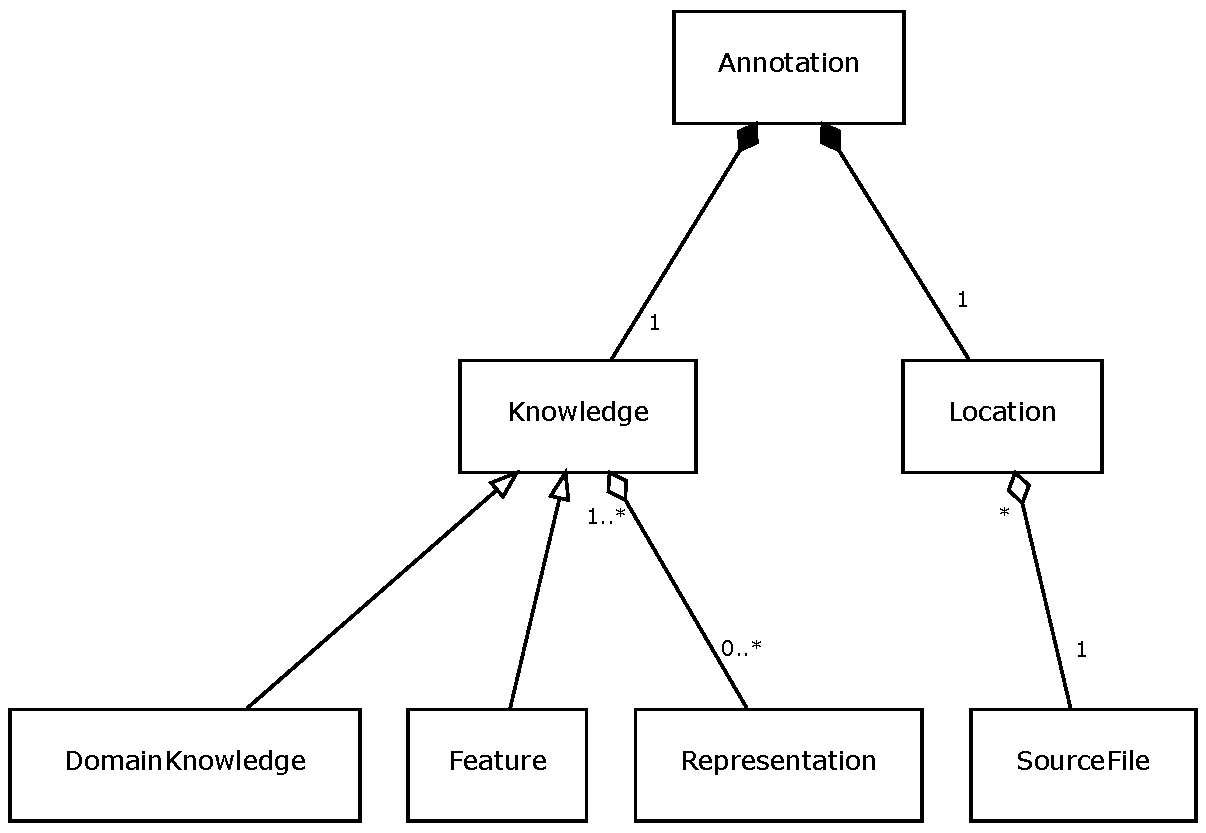
\includegraphics[width=0.75\textwidth]{../figures/sckm-upper-uml.pdf}
\caption{SCKM Annotation}\label{fig:sckm-annotation}
}
\end{figure}

\vspace{-10pt}
\hypertarget{sec:ui-formalism}{%
\subsection{Legacy User Interface}\label{sec:ui-formalism}}
\vspace{10pt}

To achieve \cref{ro:2} and \cref{ro:3}, \gls{awsm} addresses the lack of user interface migration, and user interaction reuse of existing \gls{Web Migration} approaches, as identified in \cref{g:3}.
This requires a formalism as common conceptual model for describing the \glslink{Legacy System}{legacy} user interface and its migrated derivatives.
%The user interface is an essential concern of \gls{Web Migration} since migration from a \glslink{Desktop Application}{desktop} \gls{gui} to a \glslink{web}{Web}-based \gls{gui} rendered in the browser visibly changes the ``\emph{look and feel}'' \autocite{Rodriguez-Echeverria2012MIGRARIA,Lucia2008,Distante2002} and impacts existing users.
%This formalism defines a conceptual model of the \glslink{Legacy System}{legacy} user interface that serves as the basis for the \gls{awsm} Customer Impact Control Method.
User interfaces are defined in terms of Task, Behavior, Thesaurus, Layout, and Material \autocite{Bakaev2017Kansei}.
The \gls{awsm} conceptual model of legacy user interfaces focuses on the layout aspect, because of three reasons: 1. the layout necessarily undergoes the most visible change through \gls{Web Migration}, whereas changes in e.g.~Task or Thesaurus can be avoided, 2. it is the basic design \gls{artifact} of the new \gls{web} \gls{ui}, influencing other aspects like Behavior and 3. it has the most degrees of freedom during re-design, in contrast to e.g.~Material which is governed by the platform.

\gls{awsm} defines a concrete \glslink{Legacy System}{legacy} user interface \(u \in U\) from the 
set of resources that form the user interface of the \gls{Legacy System} as
%i.e.~top-level \gls{ui} container elements without parents like screens, windows, dialogues, is defined as

\begin{equation}u = (C_u, w_v, h_v) \textrm{, where } C_u \subseteq C_{\mathfrak{L}} \textrm{ and } w_v, h_v \in \mathbb{N}_0\label{eq:ui}\end{equation}

It consists of \(C_u \), the subset of \gls{ui} controls of that particular user interface, and \(w_v\) and \(h_v\), the viewport width and height of the user interface.
%Since \glspl{gui} are rendered on raster scanned screens, the smallest unit of display is a pixel.
In \gls{awsm}, all lengths like \(w_v\) and \(h_v\) and positions are represented as non-negative integer numbers in the unit of pixel.
%
The physical size of a pixel may vary depending on the hardware.
\(C_{\mathfrak{L}} \subset T_c \times \mathbb{N}_0^4 \times C_{\mathfrak{L}}\) is the set of all \gls{ui} controls of the \gls{Legacy System} \(\mathfrak{L}\).
A \gls{ui} control \(c \in C_{\mathfrak{L}}\) is defined by its type \(t(c)\), the rectangular bounding box \(b(c)\) occupied by \(c\) within the surrounding container and its parent \gls{ui} container \(p(c)\).
%There can be a wide variety of \gls{ui} control types like labels, buttons, inputs, checkboxes etc.

\gls{ui} controls can be nested inside other \gls{ui} controls (e.g.~a button inside a form inside a window).
The nesting is represented via references to the parent: \(p: C_{\mathfrak{L}} \mapsto (C_{\mathfrak{L}} \setminus \{c\}) \cup \{0\}\).
If a \gls{ui} control contains at least one other \gls{ui} control, it is referred to as \gls{ui} container.
A \gls{ui} control \(c\) cannot be contained within itself. %Thus it is excluded from the domain of possible parents.
For root-level \gls{ui} controls \(p(c)\) is \(p(c) = 0\).
The resulting hierarchy of \gls{ui} controls forms a tree-based representation of the \gls{ui}, which is commonly used for further \gls{ui} analysis.

The bounding box \(b: C_{\mathfrak{L}} \mapsto \mathbb{N}_0^4\) is the minimal rectangular area completely enclosing \(c\) defined in terms of the horizontal coordinate \(x\) and the vertical coordinate \(y\) of the upper left corner of the rectangle and its width \(w\) and height \(h\), in pixel respectively:

\begin{equation}b(c) = (x,y,w,h) \in \mathbb{N}_0^4\label{eq:bounding-box}\end{equation}

The coordinate origin is defined as position \(x=0, y=0\) in the upper left corner of the root-level \gls{ui} container.
If a \gls{ui} control \(c\) has a parent \gls{ui} container \(p(c) \neq 0\) then the coordinates of its bounding box \(b(c) = (x,y,w,h)\) are relative to \(p(c)\), i.e.~the position \(x=0, y=0\) does not refer to the top left corner of the root-level \gls{ui} container, but to the top left corner of \(p(c)\).

%\begin{equation}c =(t_c, b, c_p) \textrm{, where } t_c \in T_c, b \in \mathbb{N}_0^4, c_p \in (C_{\mathfrak{L}} \setminus \{c\}) \cup \{0\}  \label{eq:ui-control}\end{equation}

 %\autocite{Grechanik2018,RoyChoudhary2014XPERT,Sanoja2014,Cai2003VIPS}.

%
%\begin{equation}T_c =  \{\textrm{label}, \textrm{button}, \textrm{input}, \textrm{checkbox}, \ldots\}\label{eq:ui-types}\end{equation}


%\Cref{sec:awsm-ci} describes an empirical method to measure the similarity between \glslink{Legacy System}{legacy} and \gls{web} user interfaces and a method for automatic \gls{Transformation}, based on this conceptual model.

\vspace{-12pt}
\section{Summary}
\vspace{13pt}

This chapter introduced the \gls{awsm} approach for \gls{Web Migration} initiation by \gls{sme}-sized \gls{isv} with \glslink{Legacy System}{legacy}, non-\glslink{web}{Web}, \gls{Desktop Application} products, and a large existing user base.
The basic idea of \gls{awsm} is to provide methods targeting the shortcomings of existing \gls{Web Migration} approaches in addressing doubts about feasibility and desirability within a suitable migration strategy selection of which is supported by a guided \gls{Web Migration} information system.
The approach consists of methods, tools, principles, and formalisms to facilitate \gls{Web Migration} initiation.
The three methods specify several techniques for knowledge rediscovery, \gls{risk management}, and customer impact control.
The tools of the \gls{awsm} Toolsuite provide implementations of the proposed techniques, facilitating application of the \gls{awsm} Methods and focusing on integration with migration approaches, ongoing development activities and environments. 
\gls{awsm}'s top-level design decisions reflected in four core principles promote open \gls{web} standards, integration in existing comprehensive approaches, model-driven agnosticism, and application of the \gls{Rapid Prototyping} paradigm to \gls{Web Migration}.
The formalisms provide a common basis for the \gls{awsm} Methods, their techniques and for the tools, and they include \gls{kdm}-based conceptual models of \glspl{Legacy System} and knowledge in \glspl{Legacy System}, and of a model of \glslink{Legacy System}{legacy} user interfaces.
The following three chapters provide a detailed view of the methods and tools of the \gls{awsm} Methodology and Toolsuite.